%===================================== CHAP 5 =================================
\chapter{Conjugate Bayesian Linear Q learning}{\label{ch:linear}}


In an attempt to find a better balance between exploration and exploitation this thesis investigates the use of bayesian methods to allow for Thompson sampling. This chapter builds and compares bayesian methods in a linear model context to investigate what models to use and what factors are important in a reinforcement learning setting.

\section{Linear Q learning}

In linear Q learning the goal is to create a regression model that maps the state and action to a Q-value, $Q(s,a)$. Let $x_t$ denote the state and action at timestep $t$. $X$ then denotes the design matrix containing these features and $Q$ the vector of corresponding Q-values. The regression model for a single action can then be defined as

\begin{equation}
    \label{eq:regression}
	Q(X,a) = X\beta + \varepsilon \quad \text{where} \quad \varepsilon \sim N(0,\sigma^2)
\end{equation}

with the response value defined as 

\begin{equation}
    \label{eq:q_target}
	Q(s,a) = r_t + \argmax_{a'}Q(s',a').
\end{equation}

The ordinary least squares solution to the $\beta$ coefficients can then be found using the normal equation which in matrix form is

\begin{equation*}
	\beta = [X^TX]^{-1}X^TQ
\end{equation*}

Given this model the agent can take an action by acting greedily over the models $Q(s,a)$ values in a given state. Since this is purely an exploitation strategy, it is often coupled with the $\varepsilon$-greedy policy.

\section{Bayesian Linear Q learning}

To extend linear Q learning methods to Thompson sampling a bayesian perspective is required. To do this a prior distribution is placed over the regression parameters. Using bayes rule the posterior distribution of the parameters can be calculated and used to calculate the marginal distribution over Q.

\begin{align*}
p(\theta |Q, \mathcal{F}) &\propto p(Q| \theta, \mathcal{F})p(\theta) \\
p(Q) &= \int p(Q|\theta, \mathcal{F}) p(\theta) d\theta
\end{align*}

$Q$ is a vector of all Q-values given the state $X_t$, $\theta$ denotes all parameters and $\mathcal{F}$ denotes all previous transitions. Since this is only used for Thompson sampling the value of the integral is not of interest. Instead it is the samples from $p(Q|\theta, \mathcal{F})$ that will be used to drive exploration.

\section{Conjugate Bayesian Linear Q learning}

\todo Emphasize the assumptions in this chapter

The calculation of an arbitrary posterior can be computationally heavy which is ill-suited to the already long running reinforcement learning methods. In order to keep computation costs low to this thesis will consider conjugate priors which have an analytical solution.

\subsection{Gaussian Prior with Known noise}

To start consider the model used in \cite{azziz_2018}. As in frequintist regression the noise term $\varepsilon$ is a zero mean gaussian distribution with variance $\sigma_\varepsilon$. In \cite{azziz_2018} $\sigma_\varepsilon$ is assumed known. This is rarely the case, but even if it is unknown it can be treated as a hyperparameter that has to be tuned to the environment. 

A regression model is created per action, each with the same noise variance $\sigma_\varepsilon$ and with a prior over every regression coefficient. The posterior $Q$-value for each action is expressed as 

\begin{align*}
    p(\beta_a |Q_a, \sigma_{\varepsilon_a}, \mathcal{F}) &\propto p(Q_a| \beta_a, \sigma_{\varepsilon_a}, \mathcal{F})p(\beta_a) \\
    p(Q_a|\sigma_{\varepsilon_a}, \mathcal{F}) &= \int p(Q_a|\beta_a, \sigma_{\varepsilon_a}, \mathcal{F}) p(\beta_a)d\beta_a.
\end{align*}

A common conjugate prior for the coefficients is the gaussian distribution 

$$
p(\beta_a) = \text{N}(\mu_a, \sigma_\varepsilon\Lambda_a^{-1}) 
$$

where $\Lambda_a$ is the precision matrix. With this choice of prior the posterior distribution of $\beta_a$ is still gaussian with a closed form update for the distribution parameters. Given new state-action combinations X and target action-values $Q^a$ the posterior can be updated using 

\begin{equation}
    \begin{split}
        \label{eq:known_noise_posterior_update}
        \Lambda_{a_n} & = X^TX + \Lambda_{a_0} \\
        \mu_{a_n}     & = \Lambda_{a_n}^{-1}(\Lambda_{a_0}\mu_{a_0} + X^TQ_a).
    \end{split}
\end{equation}

where the $_0$ denotes the prior and $_n$ denotes the posterior parameters. The development of these updates can be found in the appendix(\todo reference). This model will be refered to as a bayesian normal model(BN).

With this setup actions can now be picked by Thompson sampling. For each action sample $\beta$ values from its posterior distribution and a noise term from $N(0, \sigma_\varepsilon)$. These sample values are then used in the regression equation \ref{eq:regression} to get a posterior sample from $Q_a$. Finally chose the action with the highest sampled $Q$-value. 

When calculating the target $Q$-value \cite{azziz_2018} does not use $Q$-value samples. Instead the MAP estimate of $\beta$ is used which in this case is $\mu$.


\subsection{Propagating Variance}

Using the MAP estimate means that the targets are calculated by 

$$
y = r_t + \max_a X_{t+1}\mu_a.
$$

This does not correctly encorporate the target variance. To see why recall the definition of the Q-value

\begin{align*}
    Q_t &= \mathbb{E}[G_t] = \mathbb{E}[r_t + r_{t+1} + \dots] \\
    &= \mathbb{E}[r_t + Q_{t+1}] = \mathbb{E}[r_t + Q_{t+1}]
\end{align*}

This results in the regression problem $\mathbb{E}[r_t + Q_{t+1}] = X\beta_a$. However, since the expected reward is unknown this cannot be used. Instead one has access to the sample rewards from the environment. Asymptotically the mean of the samples approaches the expected value so this can be treated as a regression task with a noise term

\begin{align*}
    \mathbb{E}[r_t + Q_{t+1}] = X\beta_a \\
    r_t + Q_{t+1} = X\beta_a + \varepsilon
\end{align*}

where $\varepsilon$ accounts for the difference between the sample and the mean, $r_t - \mathbb{E}[r_t] + Q_{t+1} - \mathbb{E}[Q_{t+1}]$. This implies that the target used must be a sample from the posterior of $Q_t$ not its expected value $X\mu_a$ as used in \cite{azziz_2018}. 

The result of this is that the known noise model only includes the variance in the reward process through $r$. It does not convey the variance in the Q-value estimate of the next state. Even in a deterministic environment the policy shifts during training mean that there is an uncertainty in the Q-value of the next state. Quoting \cite{moerland_2017},  "\dots repeatedly visiting a state-action pair should not makes us certain about its value if we are still uncertain about what to do next."

Based on the above a better choice of target is

$$
y = r_t + \max_a (X_{t+1}\beta + \varepsilon)
$$

where $\beta$ is sampled from its posterior and $\varepsilon$ from the gaussian noise distribution. However the variance of $\beta$, as seen in equation \ref{eq:known_noise_posterior_update}, is independent of the target. One way to include a variance term that is dependent on the target is to include $\sigma_{\varepsilon}$ as an unknown parameter.

\subsection{Normal Prior with Unknown noise}

Including $\sigma_{\varepsilon}$ as an unknown parameter resuts in the new posterior 

\begin{align*}
    p(\beta_a, \sigma_{\varepsilon_a}|Q_a, \mathcal{F}) &\propto p(Q_a| \beta_a, \sigma_{\varepsilon_a}, \mathcal{F})p(\theta) \\
    p(Q_a|\mathcal{F}) &= \int p(Q_a|\beta_a, \sigma_{\varepsilon_a}, \mathcal{F}) p(\beta_a, \sigma_{\varepsilon_a})d\beta_a d\sigma_{\varepsilon_a}.
\end{align*}

The conjugate priors for this setup are

\begin{align*}
    & p(\sigma^2) = \text{InvGamma}(\alpha, b)          \\
    & p(\beta|\sigma^2) = \text{N}(\mu, \sigma^2\Sigma) 
\end{align*}

with the posterior update

\begin{align*}
    \label{eq:unknown_noise_posterior_update}
	\Lambda_n & = (X^TX + \Lambda_0)                                         \\
	\mu_n     & = \Lambda_n^{-1}(\Lambda_0\mu_0 + X^TQ)                      \\
	\alpha_n  & = \alpha_0 + \frac{n}{2}                                     \\
	b_n       & = b_0 + (Q^TQ + \mu^T\Lambda_0\mu_0 - \mu_n^T\Lambda_n\mu_n) 
\end{align*}

The development of these formulas can be found in the appendix (\todo reference). This model will be refered to as the Bayesian Normal Inverse Gamma model(BNIG).

\subsection{Testing Variance Propagation}

To ensure that this method is propagating uncertainty consider a simple example from \cite{osband_2018}. Consider a MPD with two states. The initial state allows only one action that deterministicly leads to state 2 with no reward. State 2 is a terminal state with a known posterior distribution. If a RL method properly propagates uncertainty the posterior distribution of state 1 should match state 2 as long as $\gamma=1$. 

Both models were tested with both MAP and sample targets. The priors for the BN models were set to

\begin{align*}
    \beta &\sim N(0,10^3)\\
    \sigma^2 &= 1
\end{align*}

and the priors for the BNIG models were set to

\begin{align*}
    \beta &\sim N(0,10^3) \\
    \sigma^2 &\sim InvGamma(1,1).
\end{align*}

Three MDP's were set up with a known posterior of $N(1, 0.1), N(1, 1)$ and $N(1, 10)$ respectively. The results are seen in figure \ref{fig:proptest}.

\begin{figure}[H]
    \centering
    \subfloat[$N(1,0.1^2)$]{
        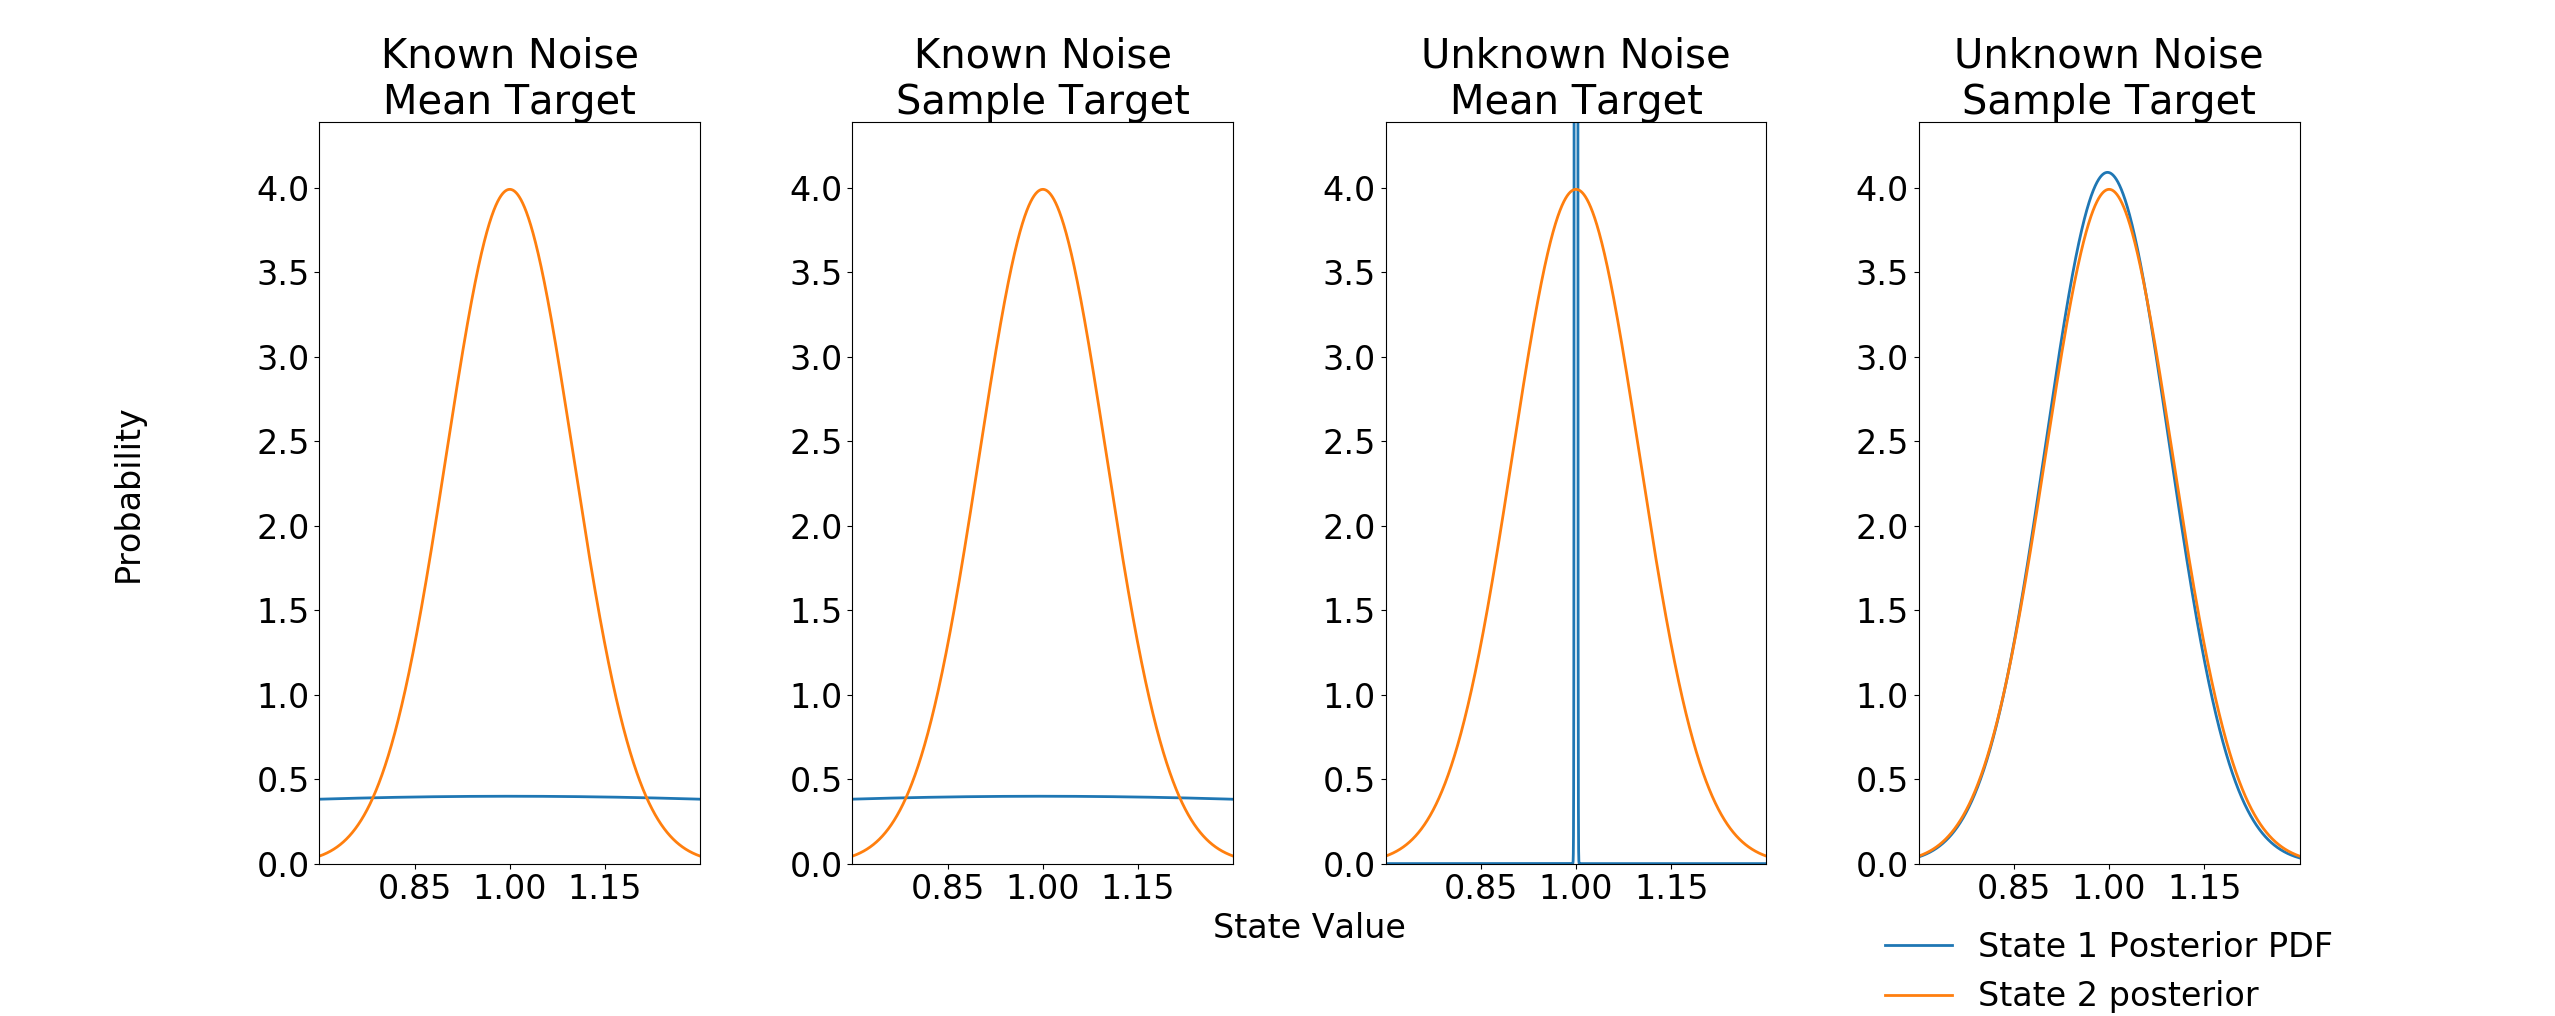
\includegraphics[width=0.6\textwidth, height=0.15\textheight]{1000iterationsSD01.png}
    }
    \\
    \subfloat[$N(1,1^2)$]{
        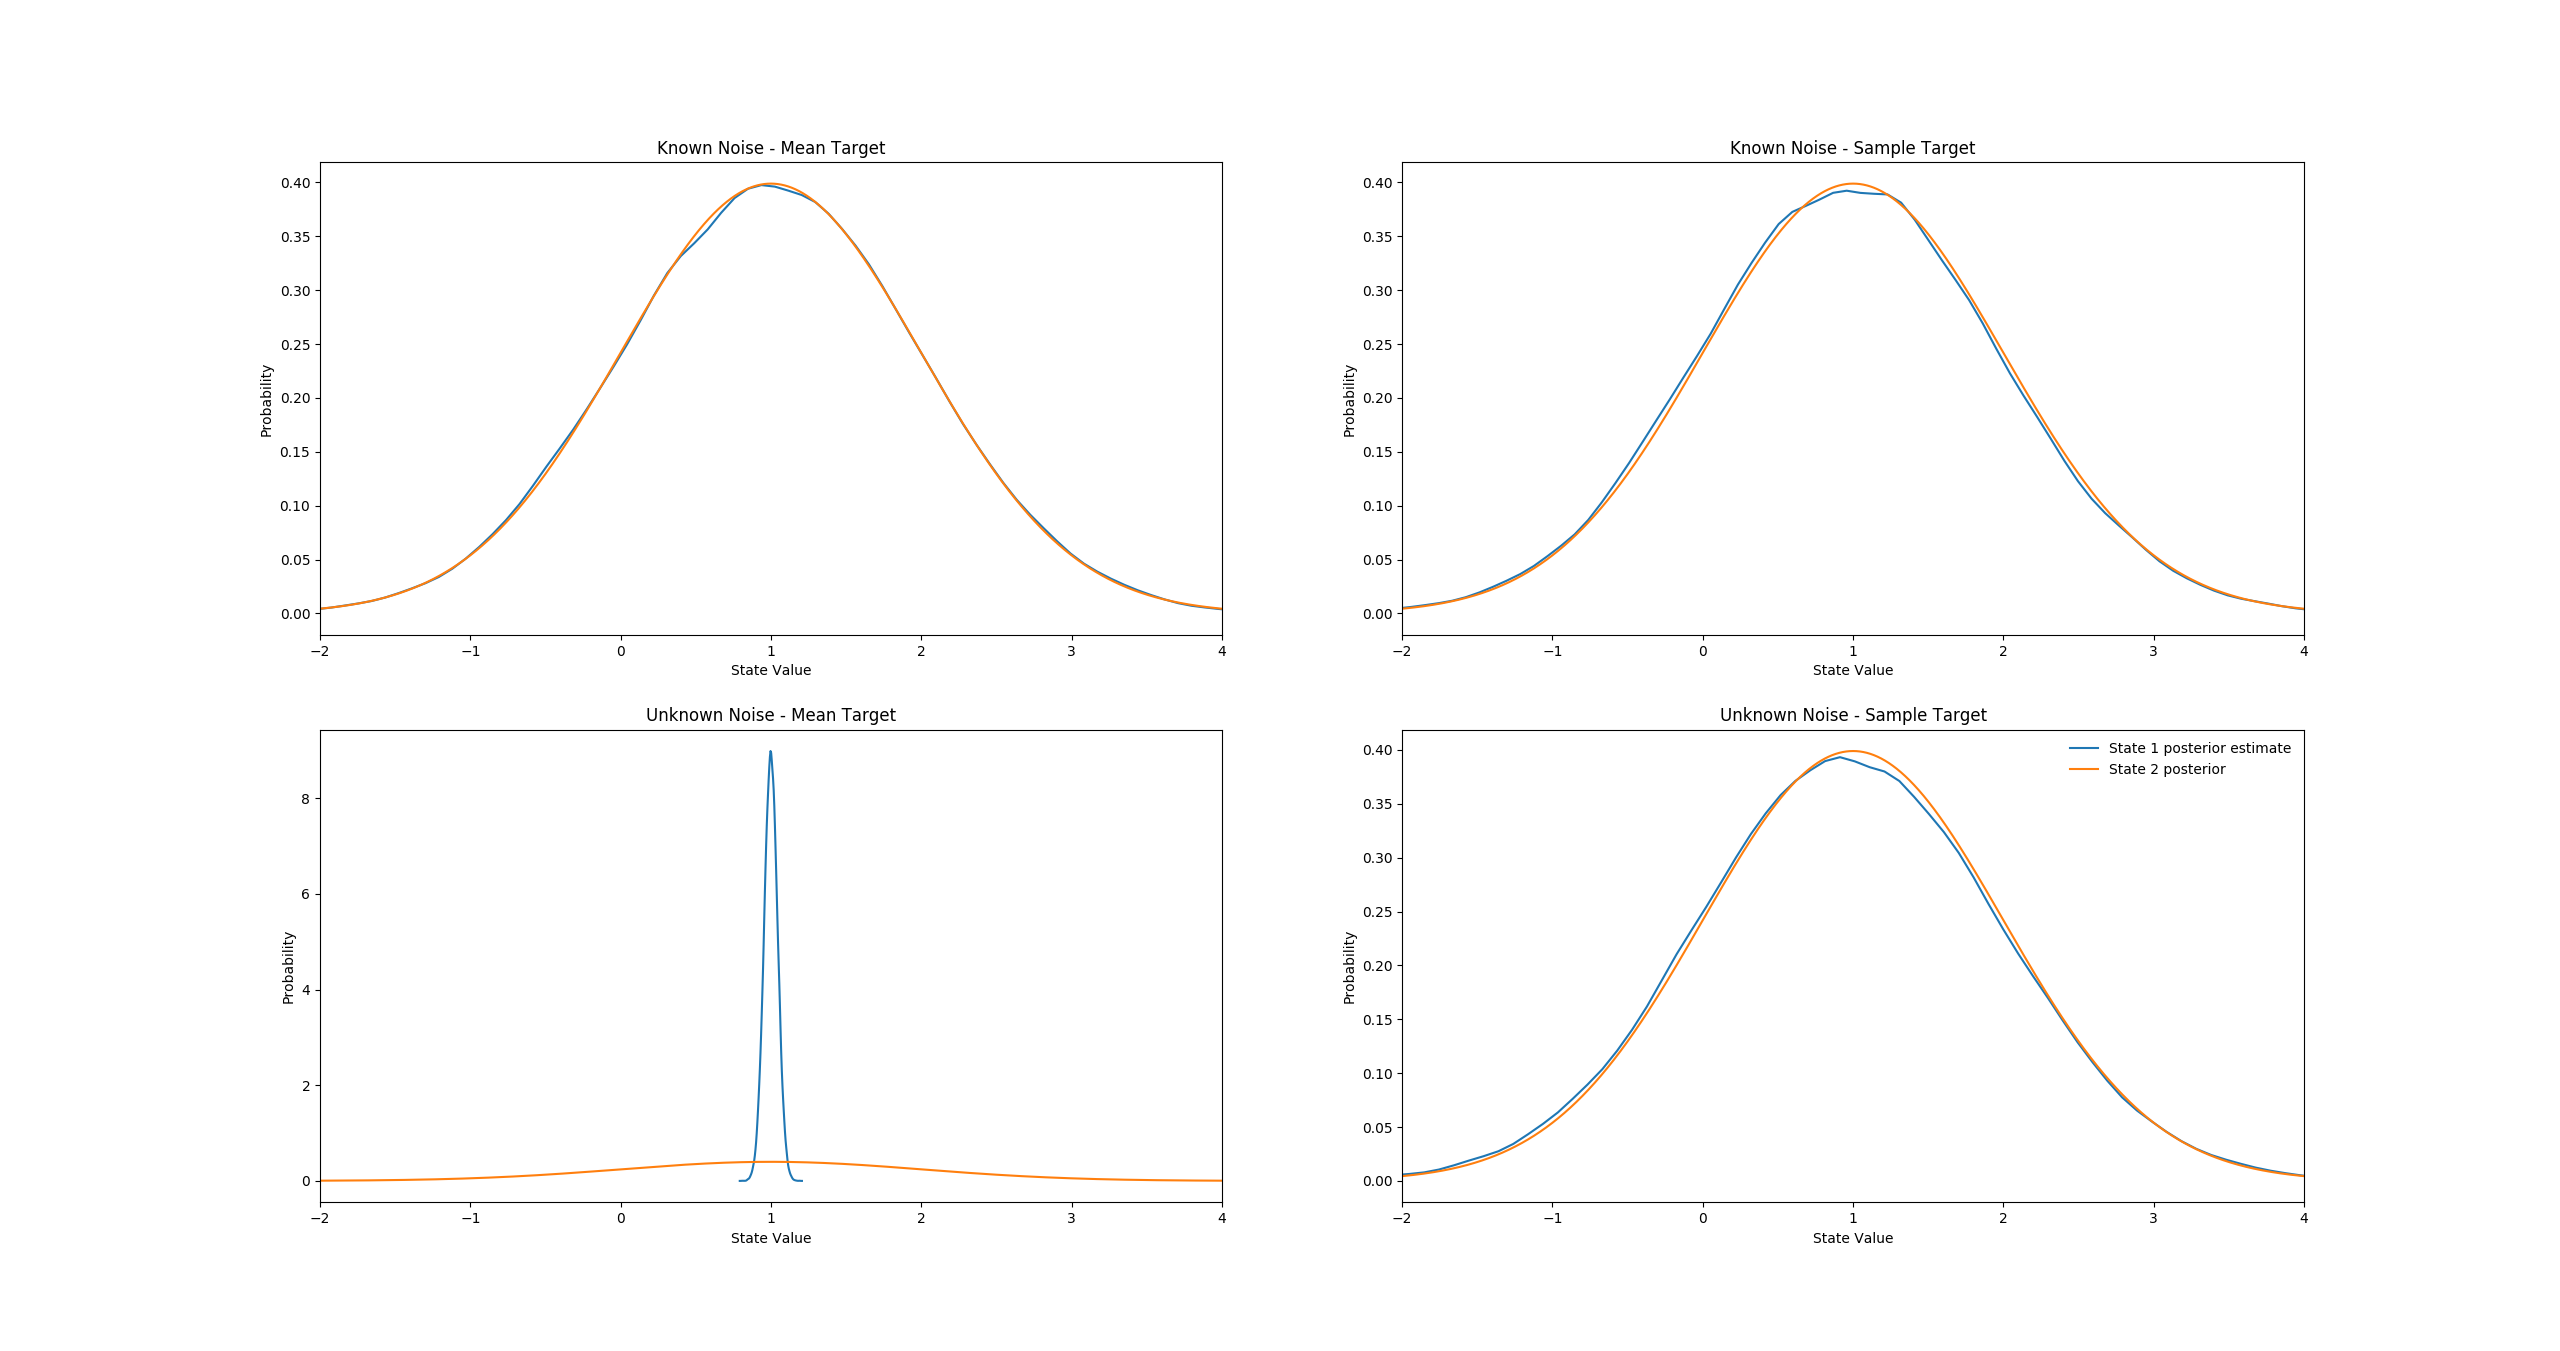
\includegraphics[width=0.6\textwidth, height=0.15\textheight]{1000iterationsSD1.png}
    }
    \\
    \subfloat[$N(1,10^2)$]{
        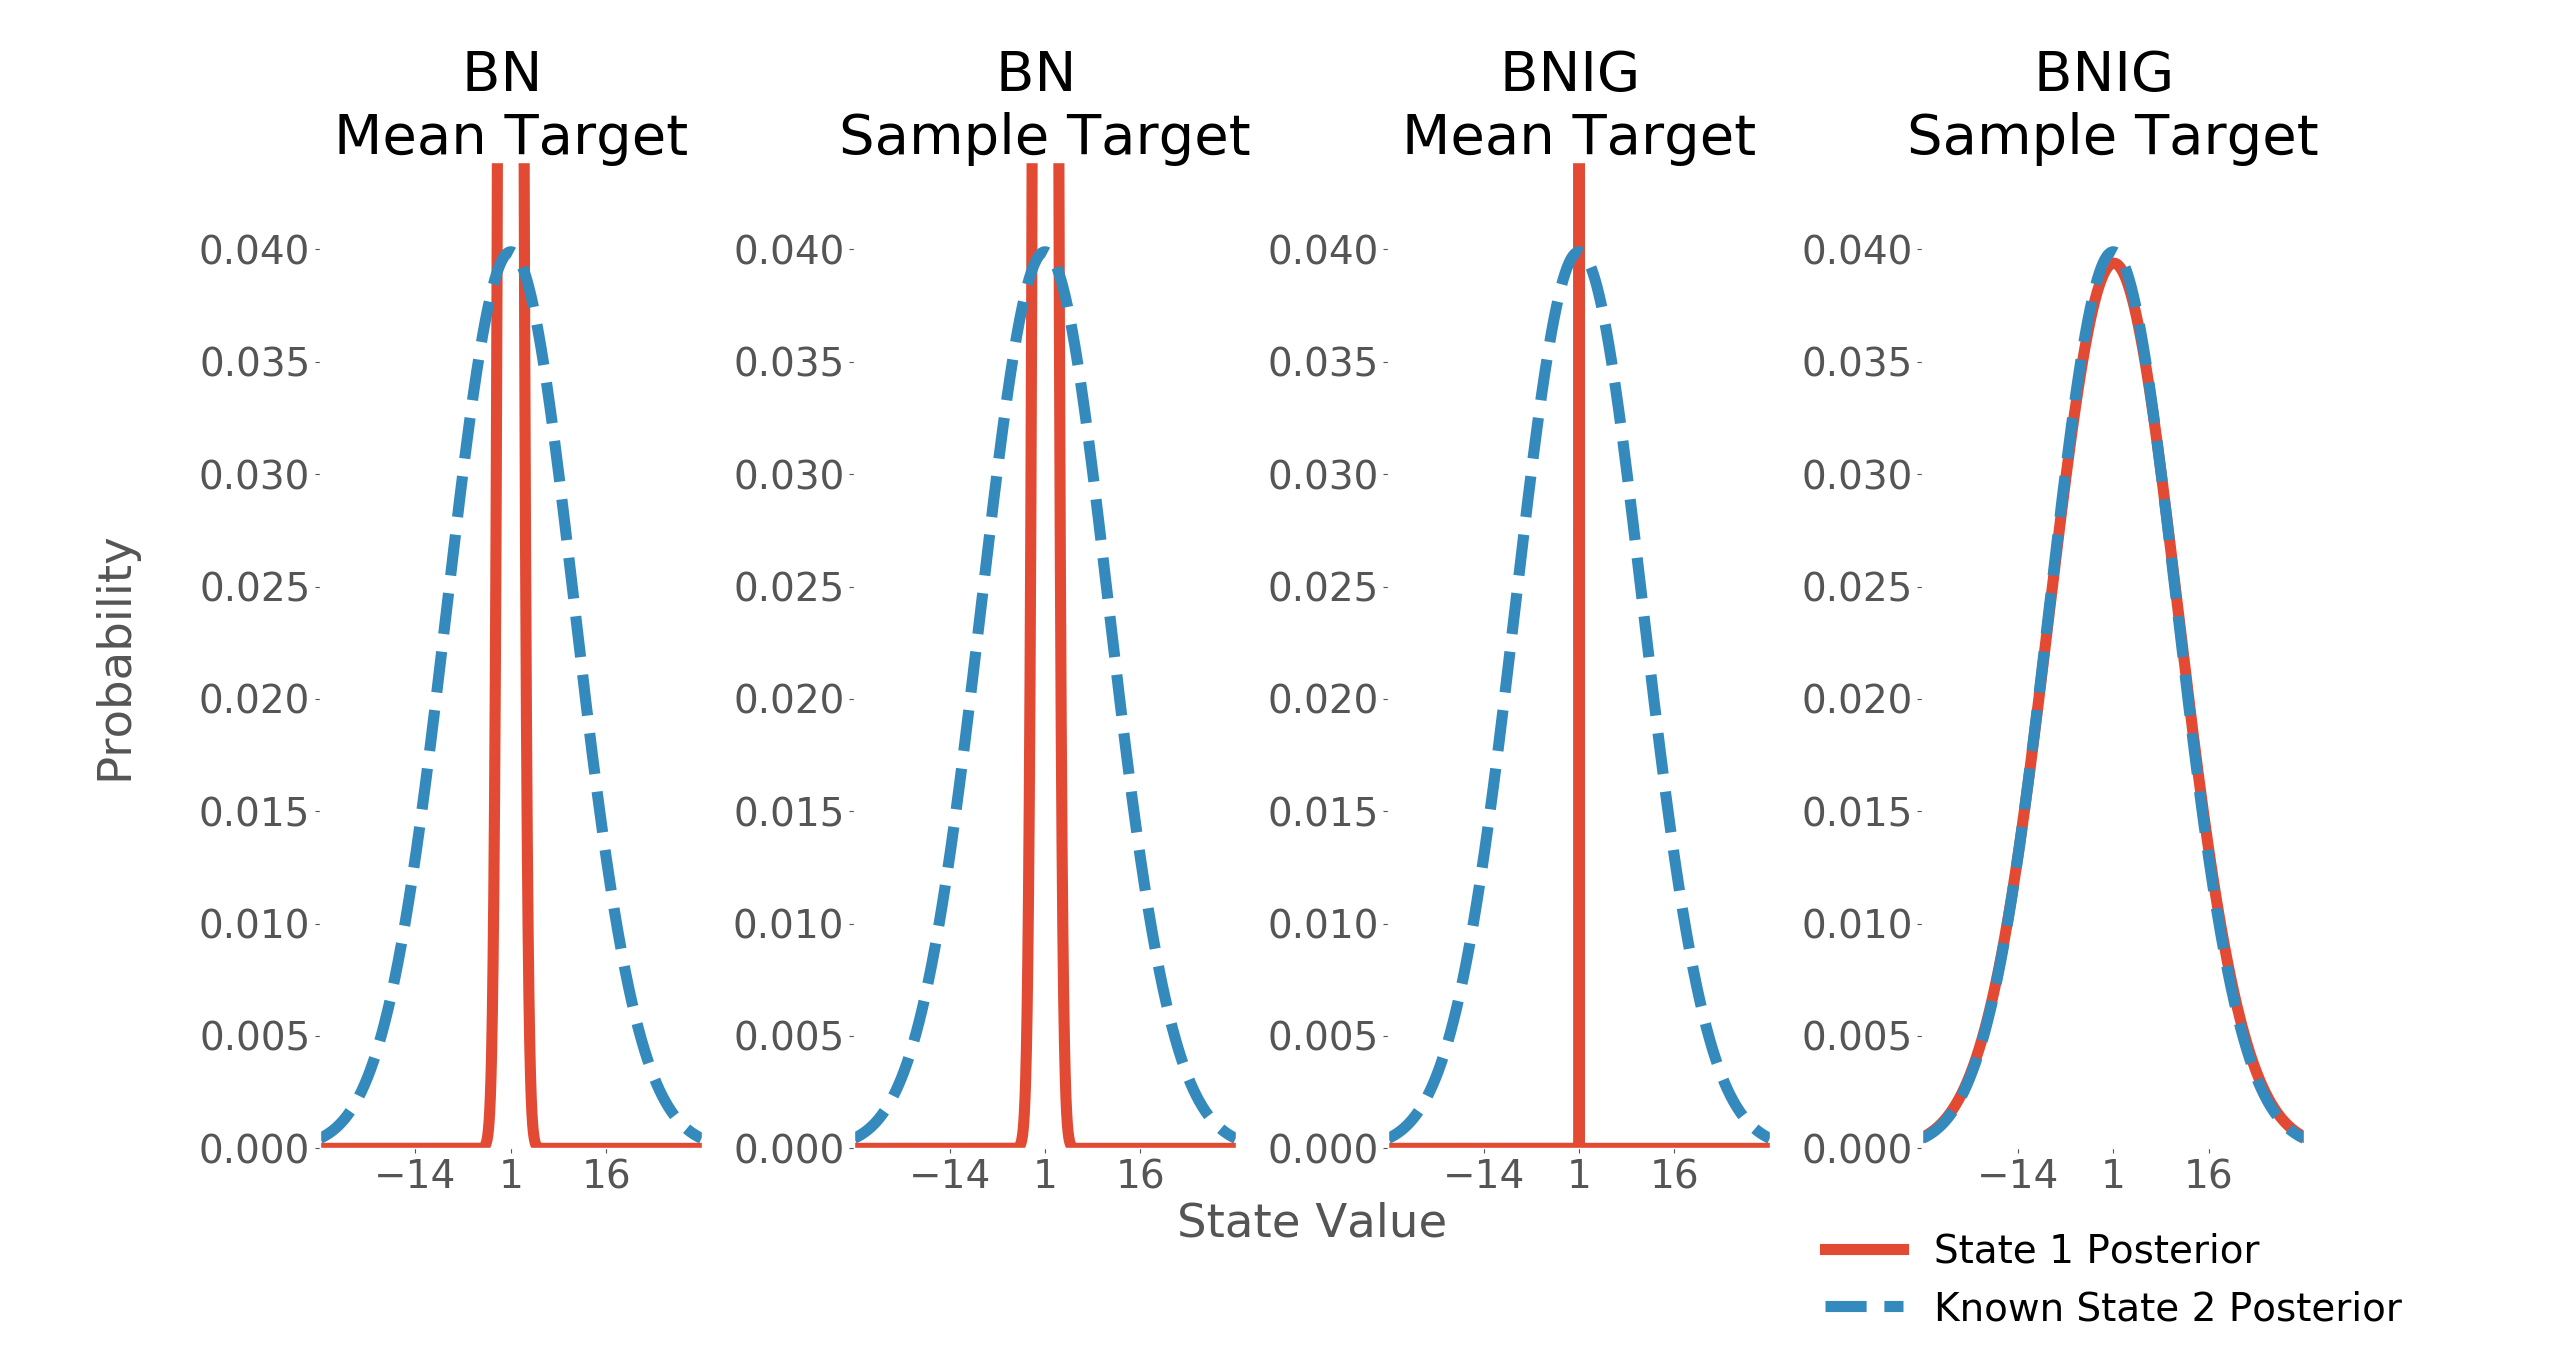
\includegraphics[width=0.6\textwidth, height=0.15\textheight]{1000iterationsSD10.png}
    }
    \caption{\textbf{Variance Propagation On 2 State Toy Example}: The blue lines show the models Q-value posterior distribution while the orange lines show the target posterior distribution. Only the BNIG model with sample targets is able to correctly estimate the target in all cases.}
    \label{fig:proptest}
\end{figure}

The results summarized in figure \ref{fig:proptest} showed that all models were able to correctly estimate the mean. However the target variance was only correctly estimated by the the BNIG model with sample targets. The BNIG model with the MAP target leads to the correct mean but dramatically understimates the variance. This would be an expected result if the model is approximating $\mathbb{E}[Q]$ instead of $Q$. The BN model is only correct for both the mean and sample target if the hyperparameter $\varepsilon$ is set to the correct variance. In an unknown and more complex environment this is unlikely to be possible. However with enough hyperparameter tuning one could argue that this can lead to good results which might explain the results achieved in \cite{azziz_2018}.

Based on these results further developments are focused on the BNIG model with sampled targets.

\section{Variance Propagation}

\subsection{Over Multiple States}

The setting above is equivalent to regular regression. In a RL setting the variance needs to be propagated to further states. To test that this is still the case with the BNIG model consider a modification to the environment where an extra state is placed between the initial and terminal state. This state has the same dynamics as earlier. It deterministically transitions to the next state with zero reward over the transition. The correct posterior for each state is then the target posterior in the terminal state. 

The same priors as earlier are used on 4 different target posteriors. The results are summarised in figure \ref{fig:3stateproptest}.

\todo Add details around these experiments in the appendix

\begin{figure}[H]
    \centering

    \subfloat[$N(1,1^2)$]{
        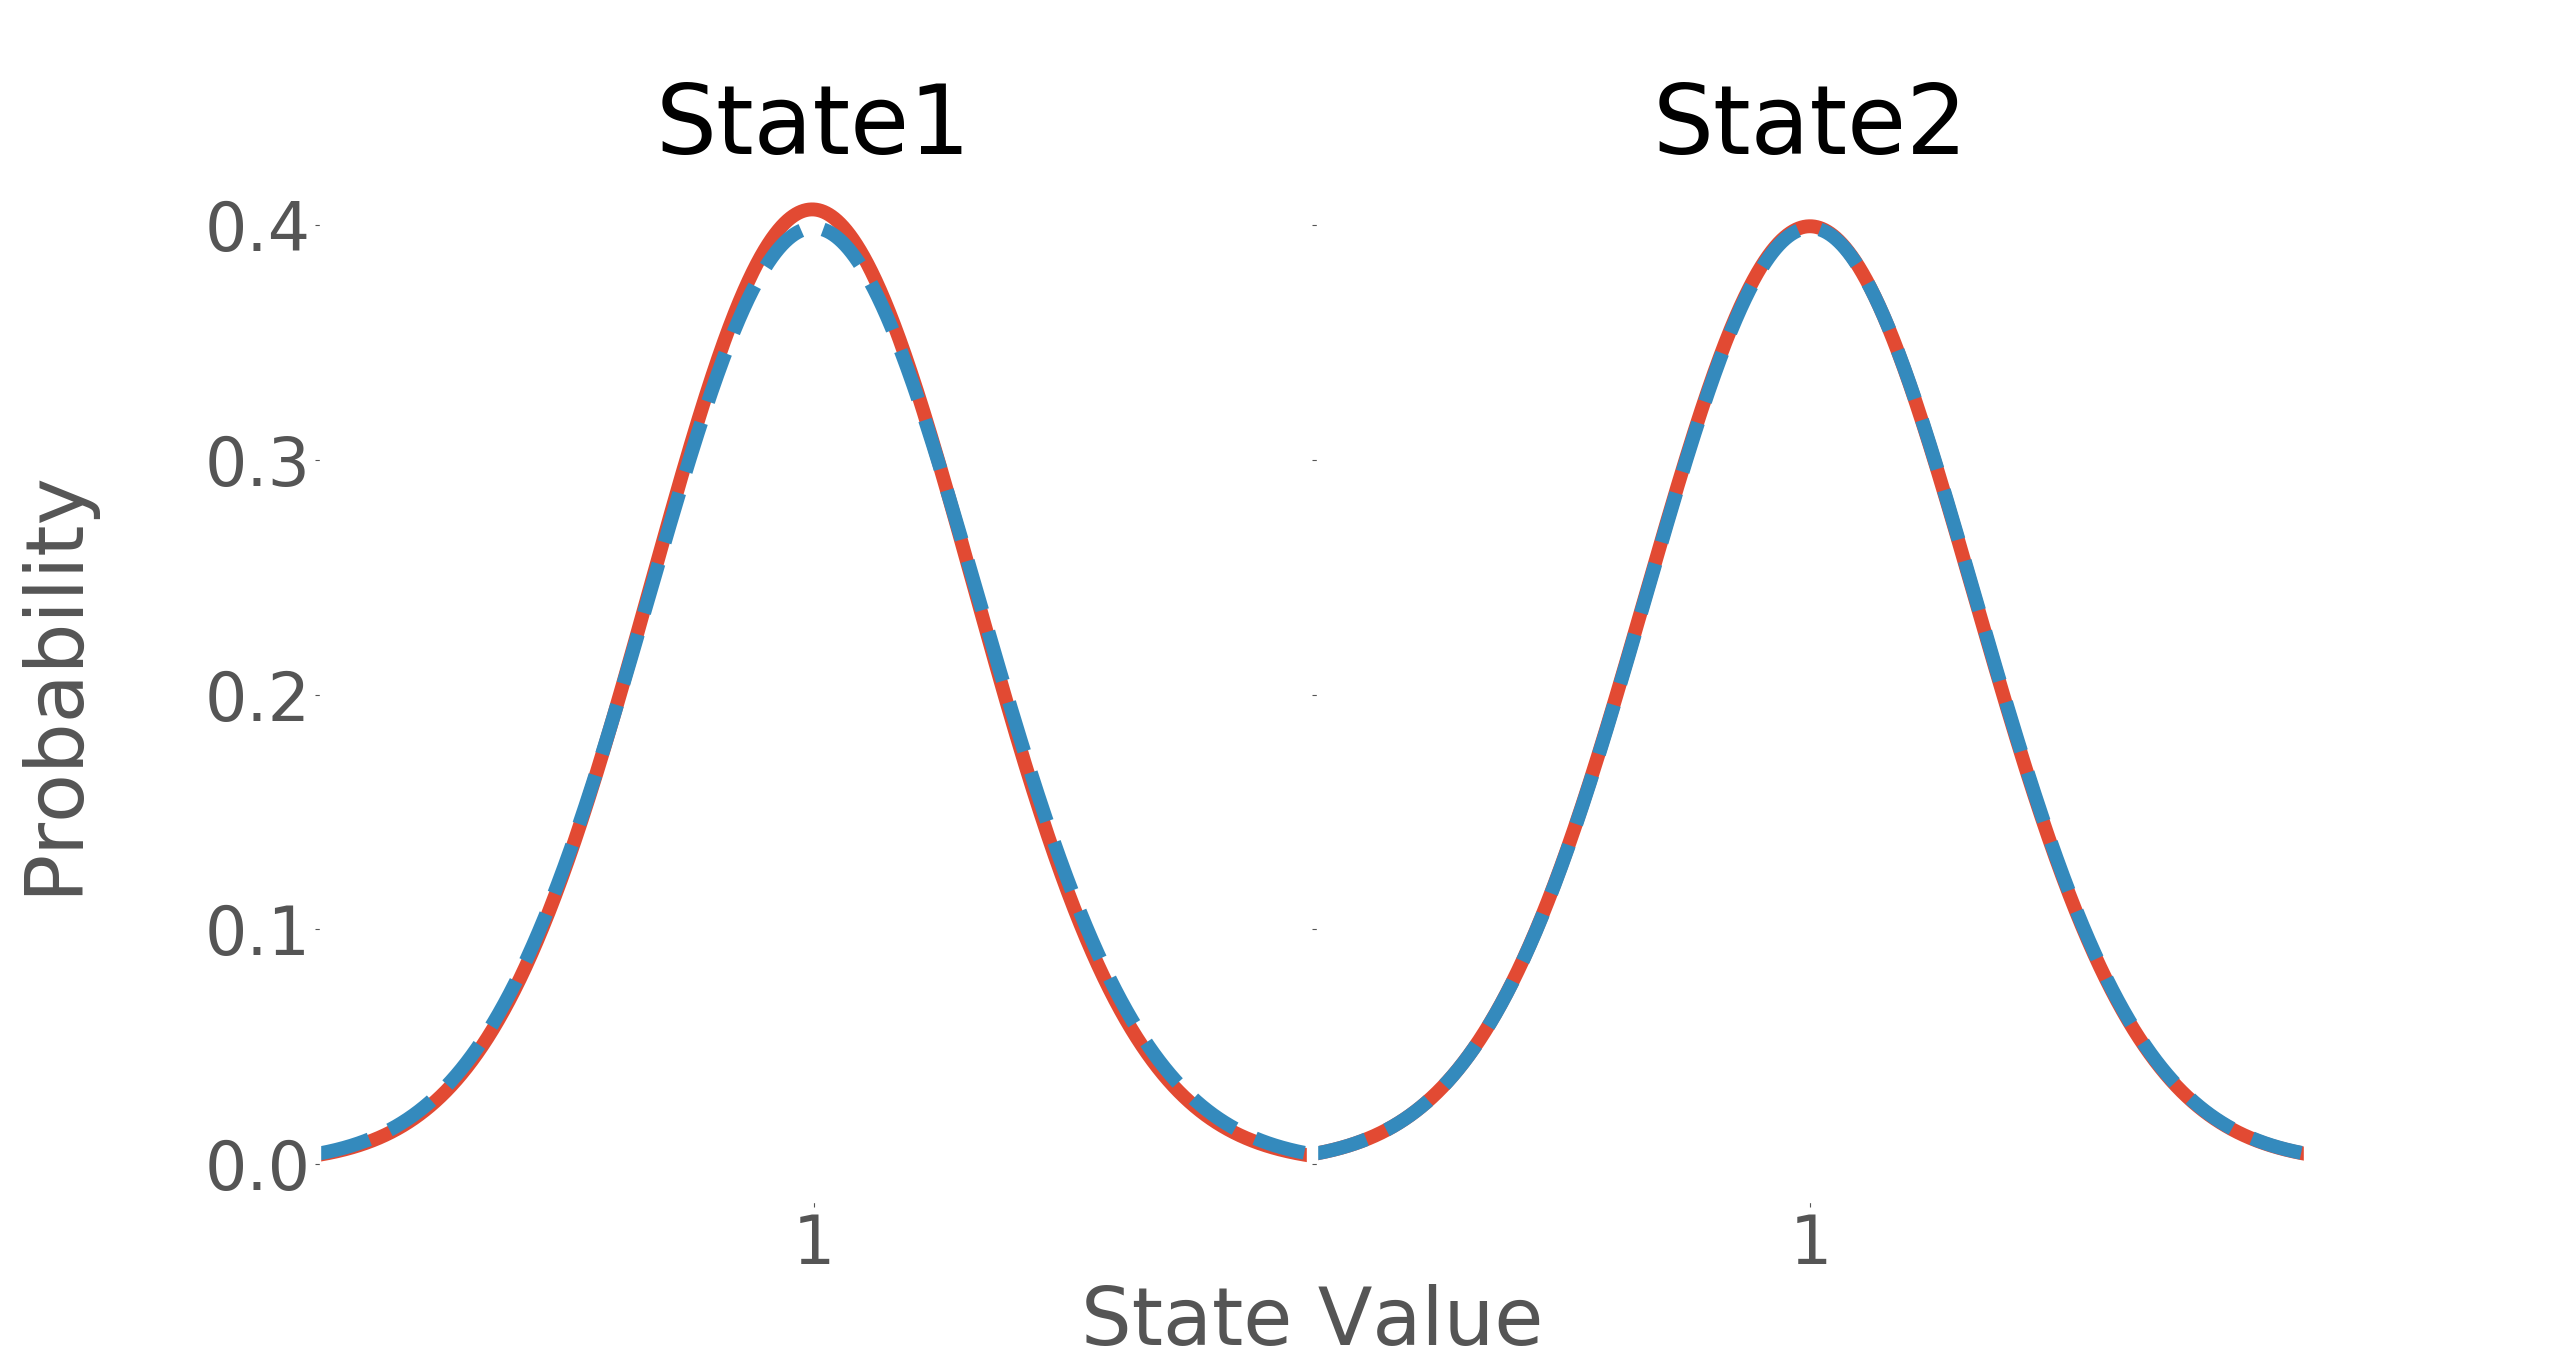
\includegraphics[width=0.45\textwidth]{3State10000iterationsSD1.png}
    }
    \subfloat[$N(1,10^2)$]{
        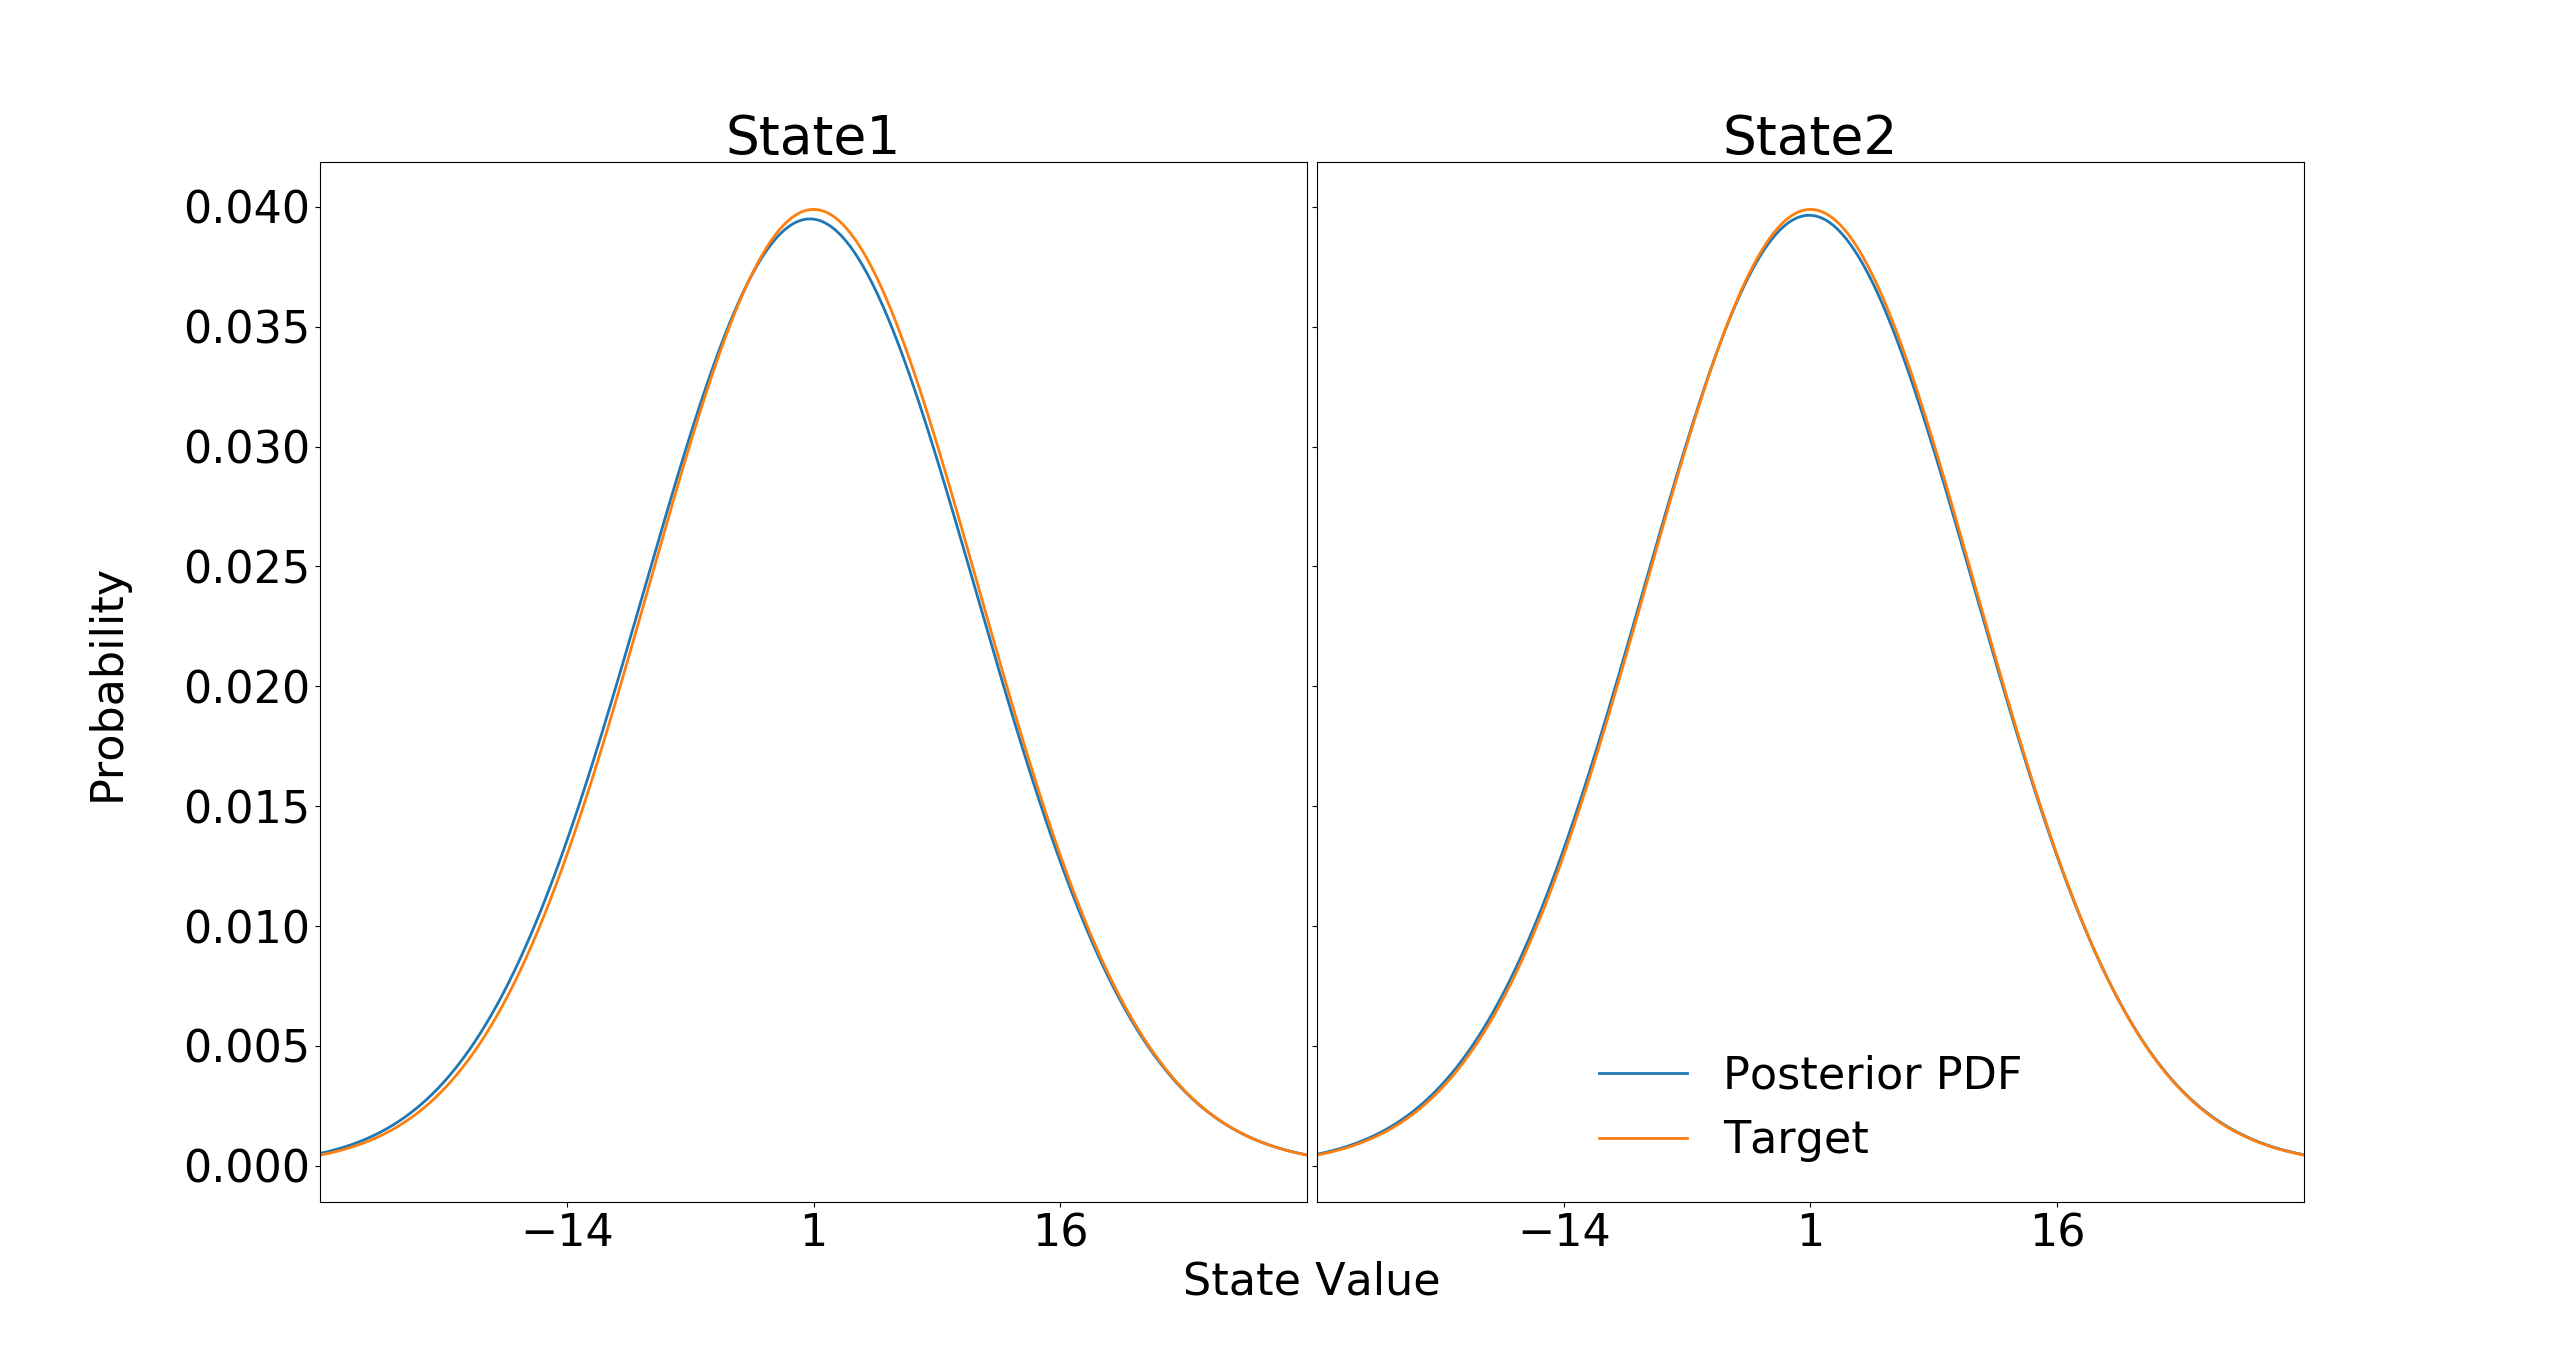
\includegraphics[width=0.45\textwidth]{3State10000iterationsSD10.png}
    }
    \\
    \subfloat[$N(1,0.1^2)$]{
        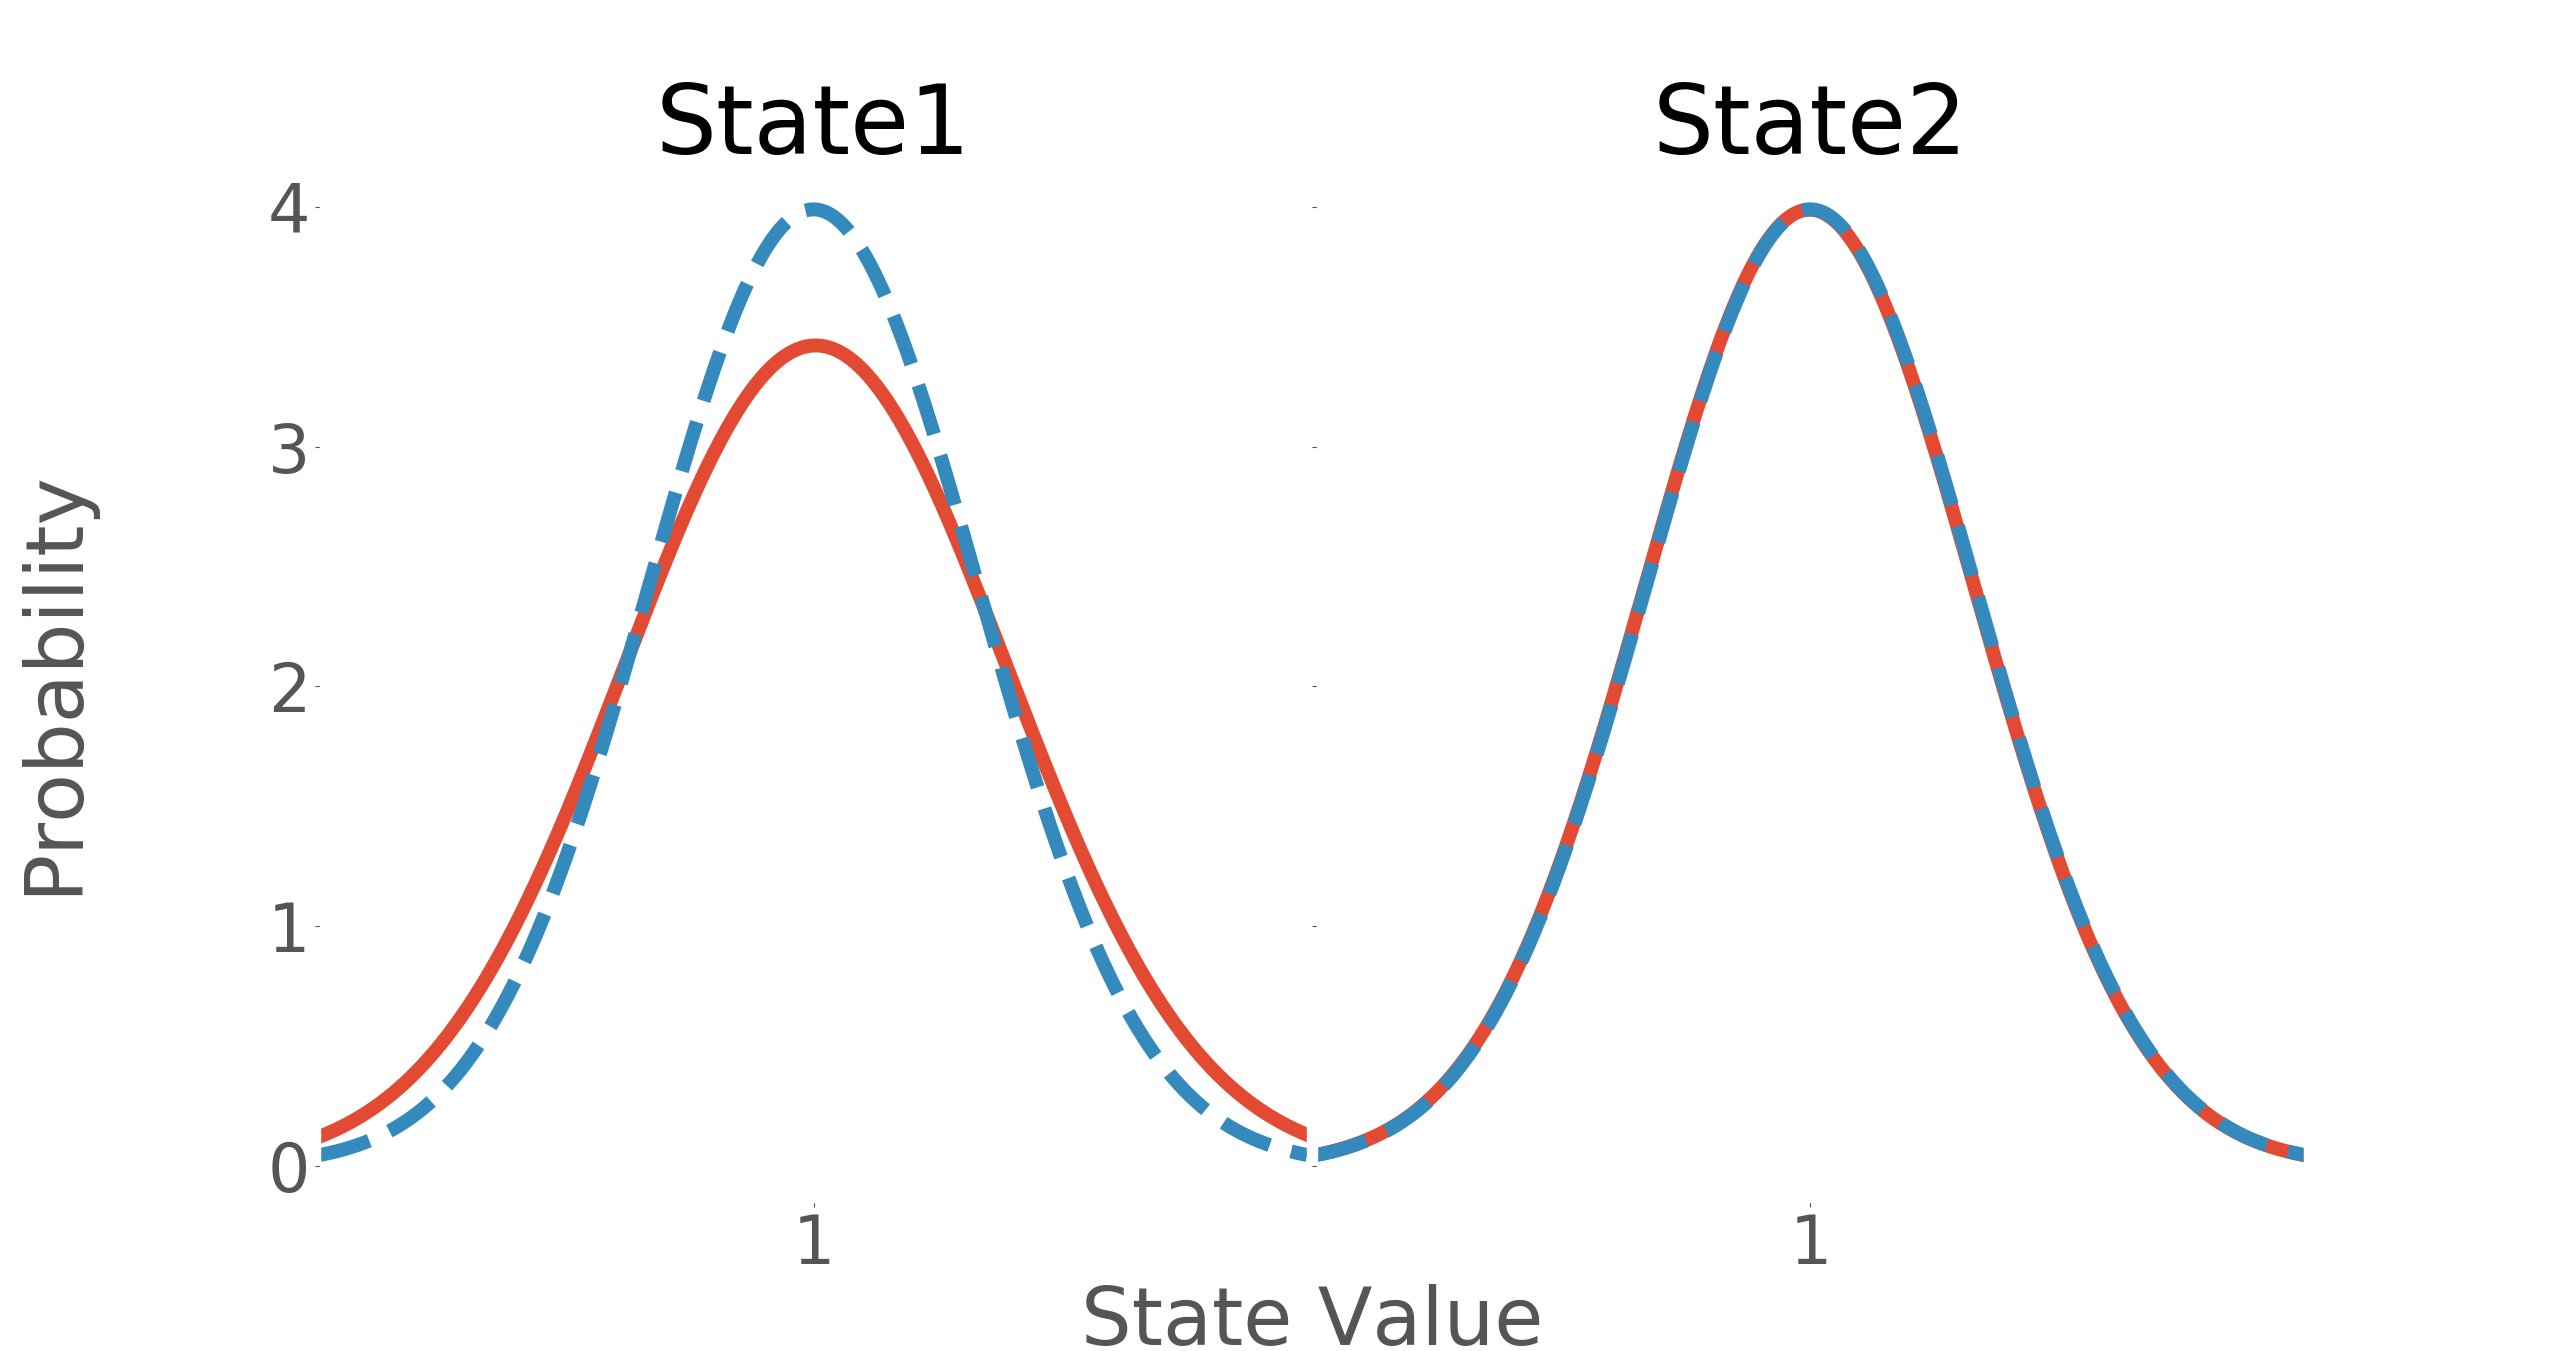
\includegraphics[width=0.45\textwidth]{3State10000iterationsSD01.png}
    }
    \subfloat[$N(1,0.01^2)$]{
        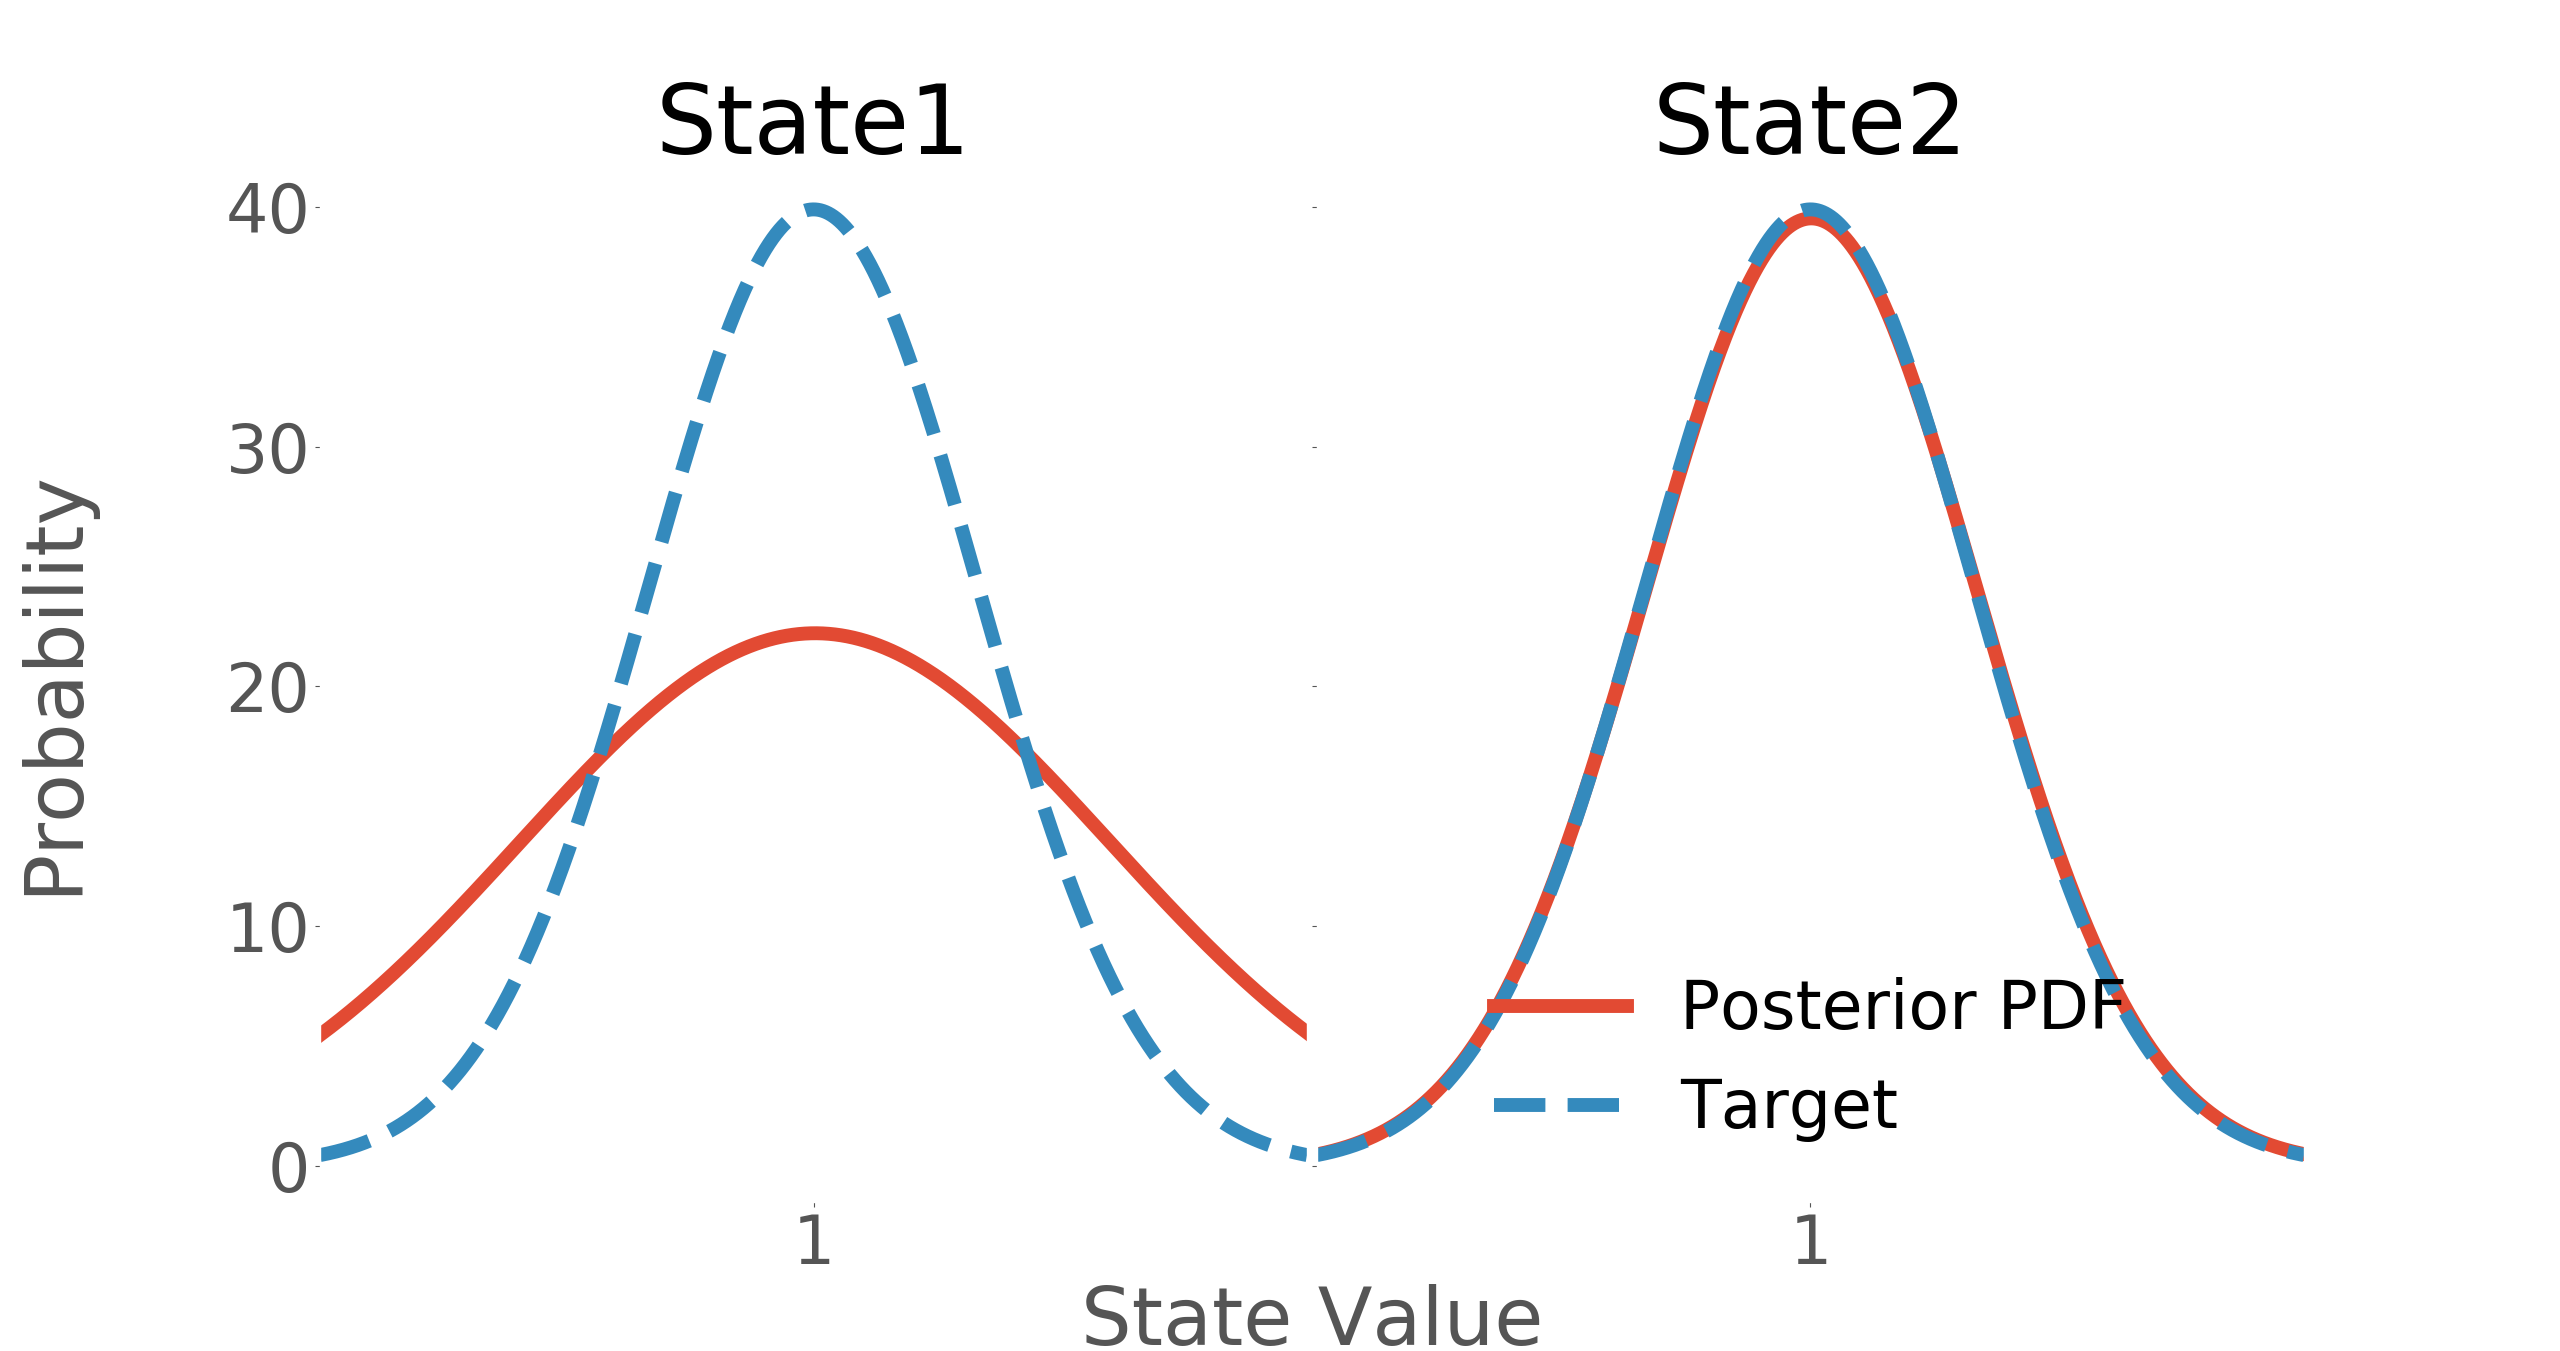
\includegraphics[width=0.45\textwidth]{3State10000iterationsSD001.png}
    }
    \caption{\textbf{Variance Propagation On 3 State Toy Example}: The models posterior estimate for the two first states are shown. The third state is the terminal state that returns a sample from the target distribution.}
    \label{fig:3stateproptest}
\end{figure}

Figure \ref{fig:3stateproptest} shows that for larger variance targets the propagation correctly updates the state 1 variance. However the low variance targets results in an overestimation over the variance in state 1. Running this experiment for more iterations does lead to a better approximation implying that the problem lies in the the convergence rate for different posteriors. 

One possible reason for this is that the posterior representing the 0.01 standard deviation posterior is more sensitive to small changes in in its parameters than the larger variance posteriors. In other words small changes in the parameters for a distribution with low variance leads to large changes in the variance of the posterior. Since the learning is happening in an online fashion the first estimates of the posterior will likely have large error. This effect is amplified for state 1 since it is training on the large error state 2 posterior. (\todo: Confirm/source that this is actually the case)

By extending the toy example to even more states as in figure \ref{fig:longproptest} one can see that this problem increases the further the variance needs to be propagated. Even large variance targets will fail to correctly propagate given enough states.

\begin{figure}[H]
    \centering
    \subfloat[6 States with $N(0.1,1^2)$]{
        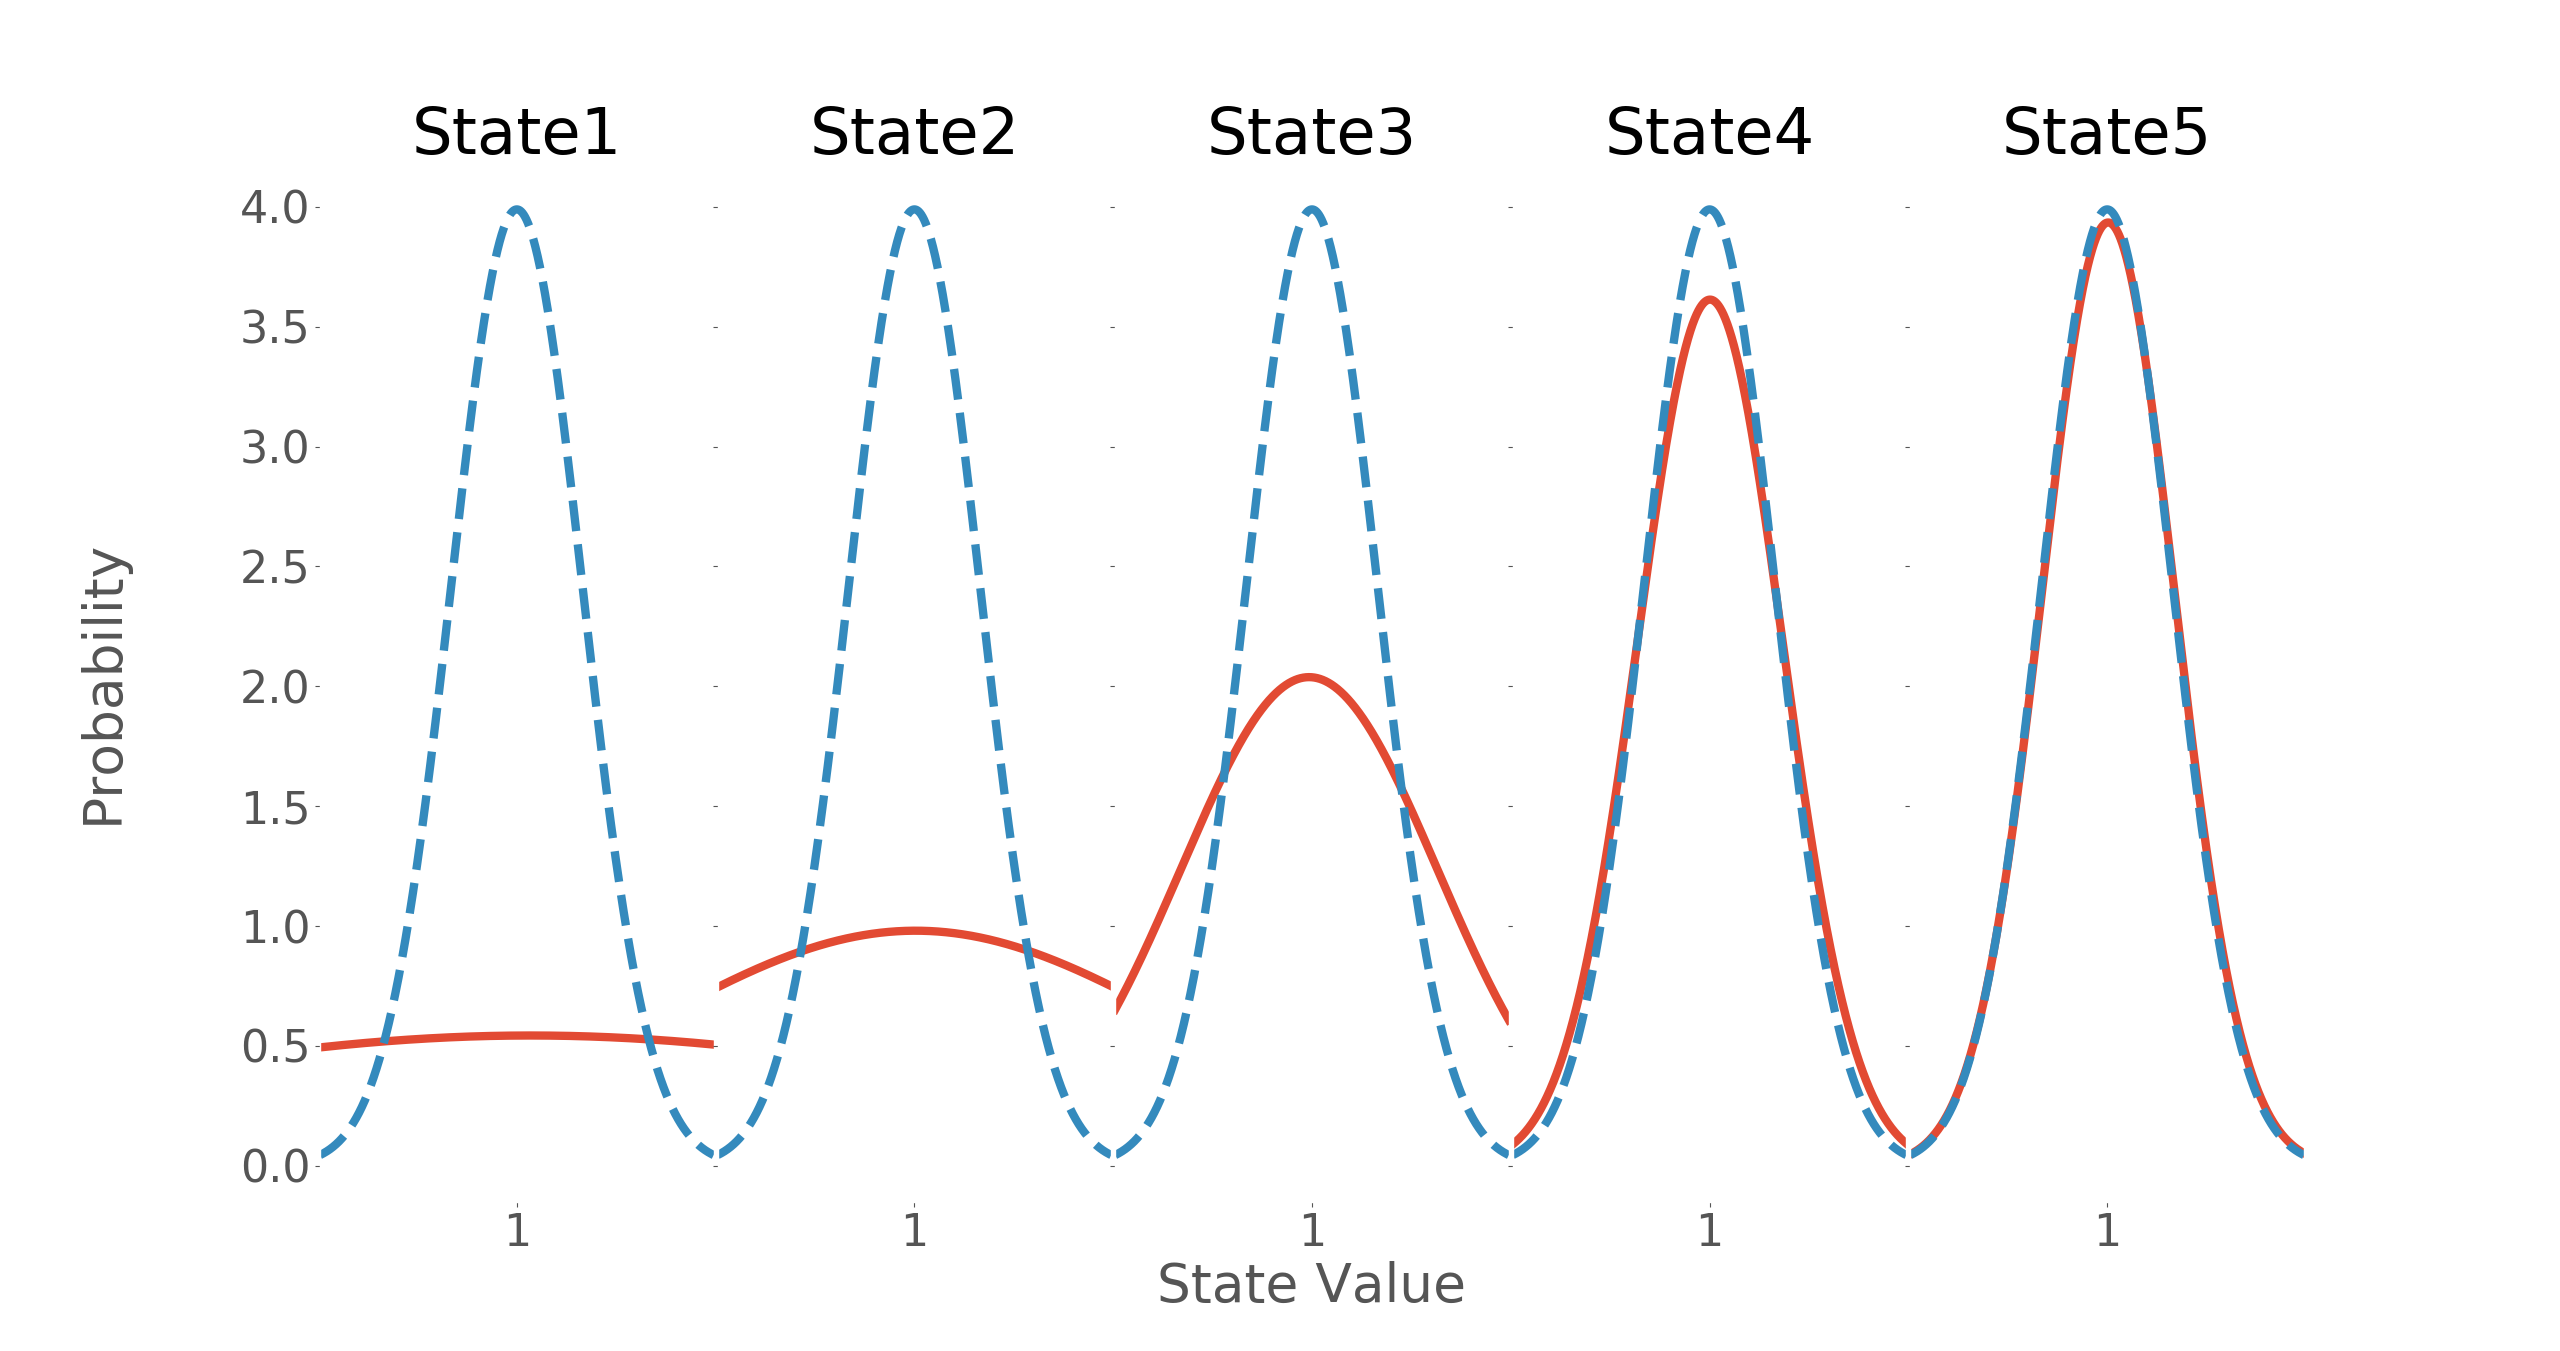
\includegraphics[width=0.7\textwidth]{6State1000iterationsSD01.png}
    }
    \\
    \subfloat[6 States with $N(1,1^2)$ target]{
        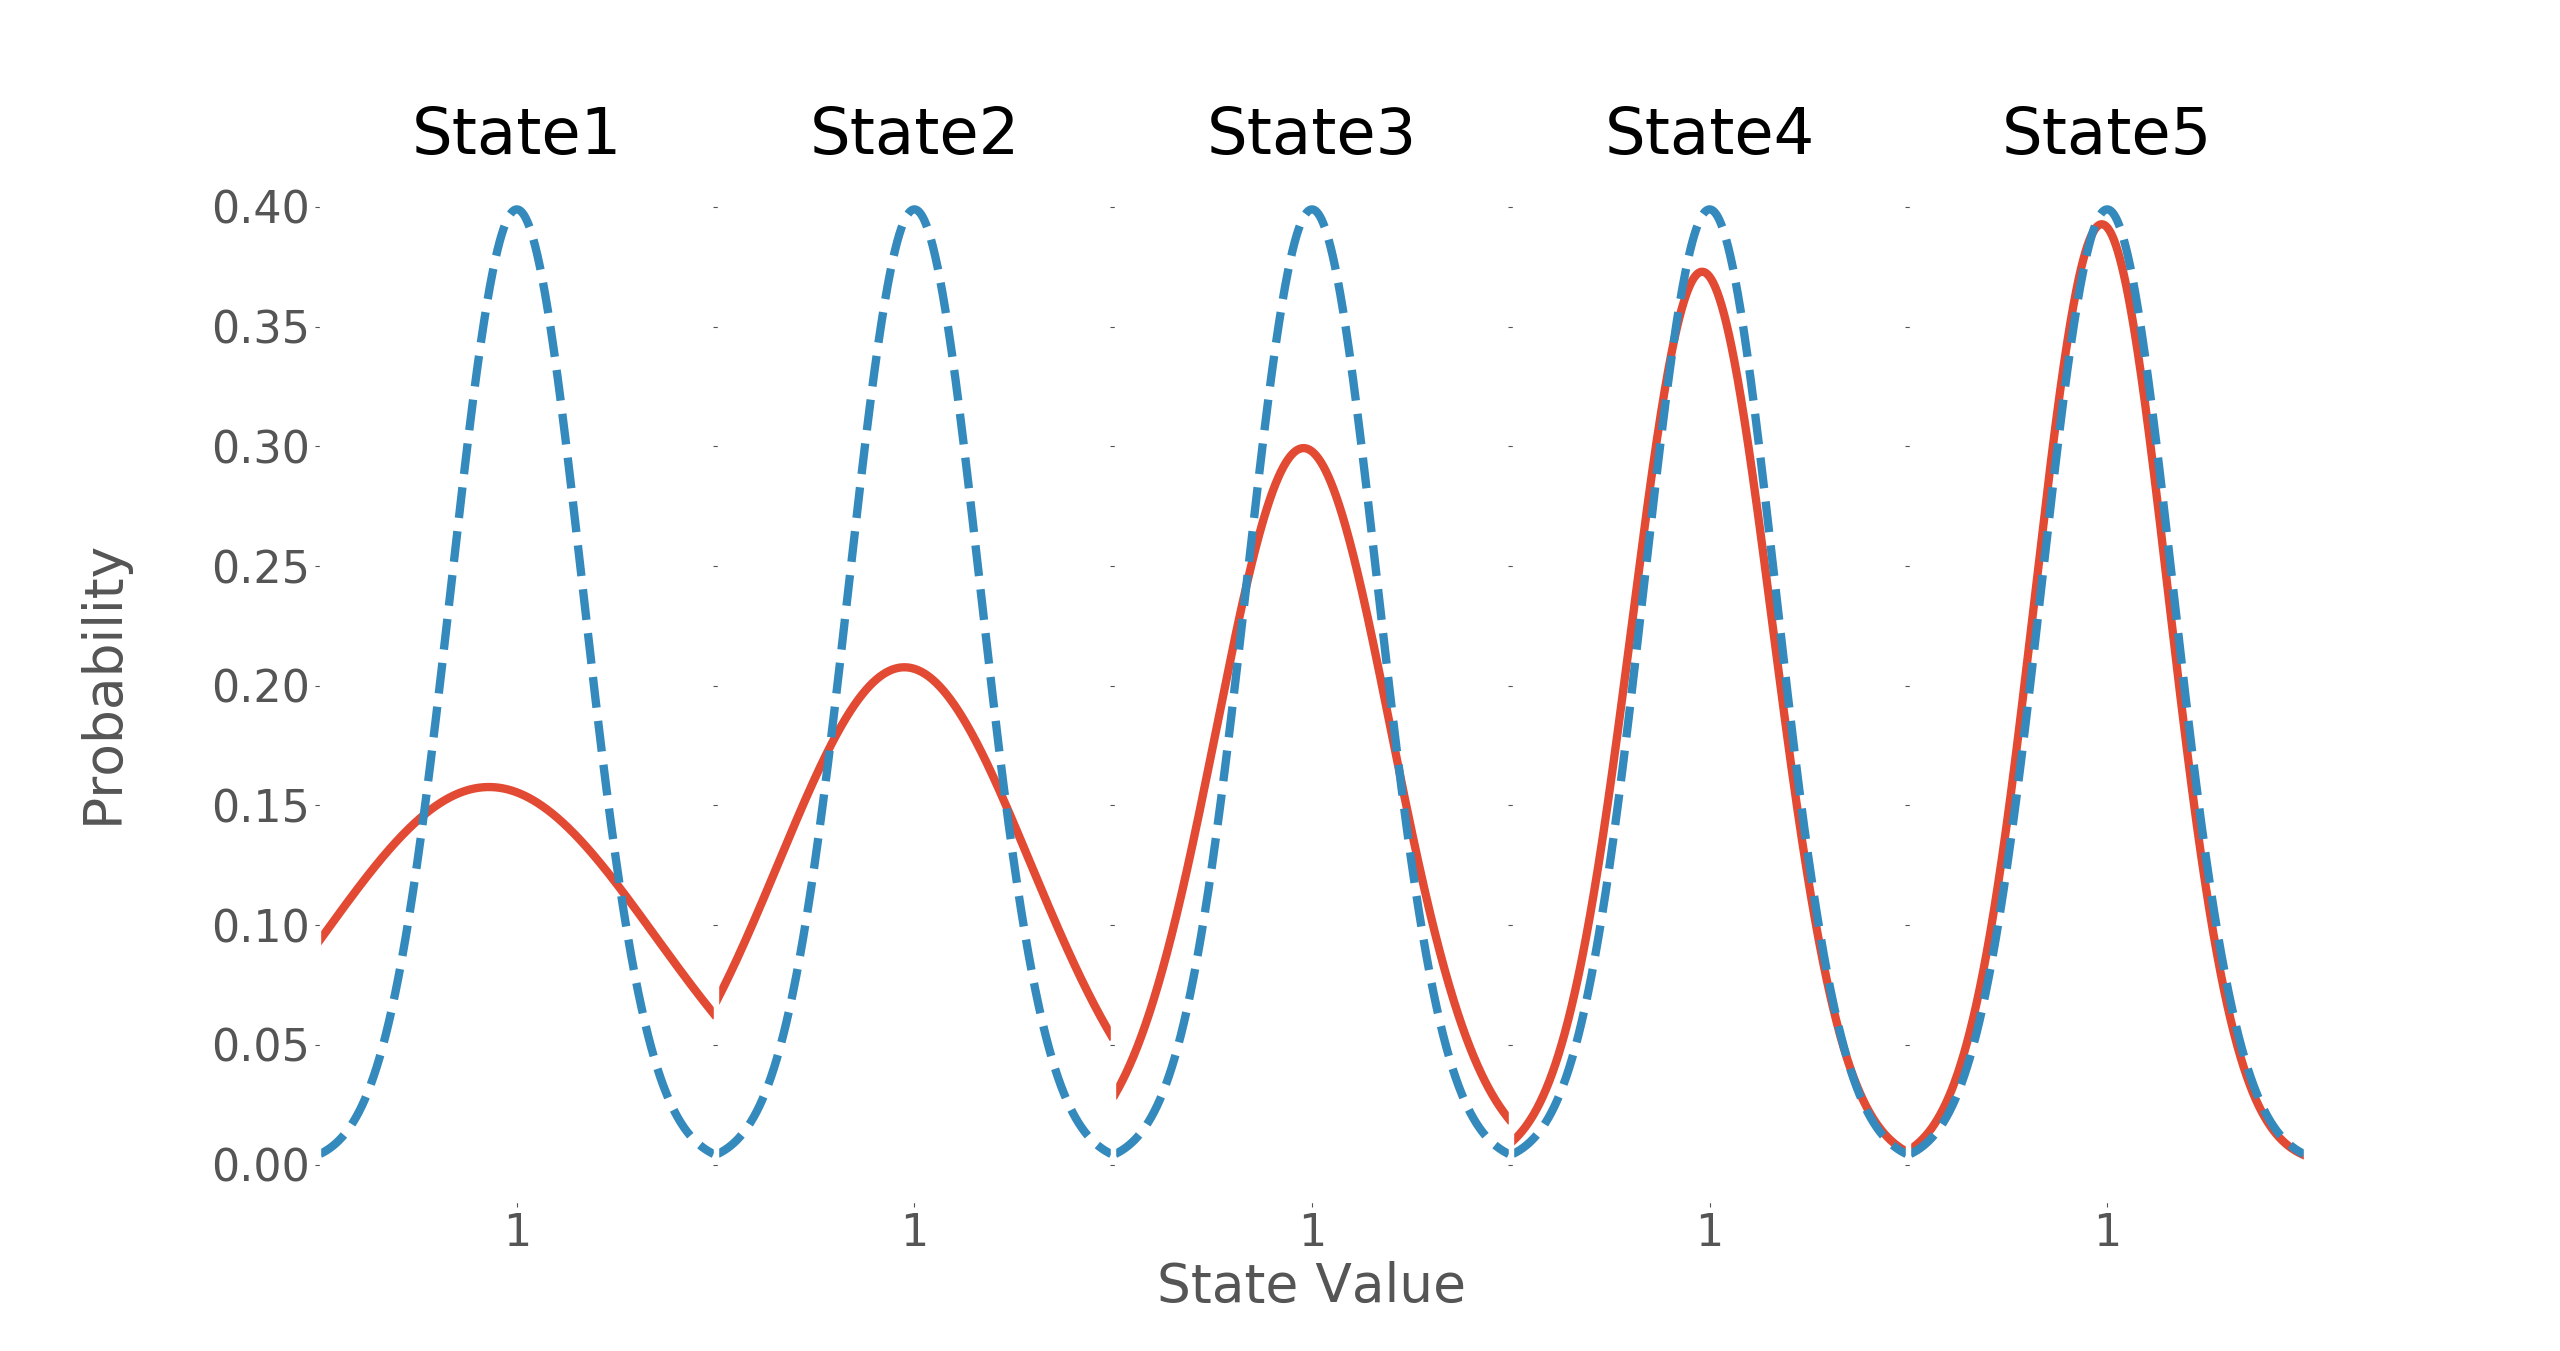
\includegraphics[width=0.7\textwidth]{6State1000iterationsSD1.png}
    }
    \caption{\textbf{Failure of variance propagation over many states}: (\textbf{a}) shows that the error in estimation close to the terminal state leads to failure in the estimation of the posterior of the initial states. In (\textbf{b}) the seemingly correct estimation close to the terminal state still does not prevent errors closer to the initial state.}
    \label{fig:longproptest}
\end{figure}

This issue will be refered to as the speed of propagation. It encompasses the problem of quickly propagating variance estimates from downstream states back to states which are far from the environments reward.

\todo: Define speed of propagation. Maybe a seperate subsection that plots how the error changes with length of chain. How do we measure the error between two distributions? KL Divergence?

\subsection{Speed of propagation}

Inorder to improve the speed of propagation insight is required into what causes the issue. In this section two causes and methods for counteracting them are discussed. However these are not necessarily the only two causes of slow propagation.

\todo These argumentations are weak and require sources or "proof". 

The first cause is best explained using an example. Consider the 3 state toy example. State 1 can only converge to the correct distribution once State 2 has converged. If more states are added, State 1 will only converge once all the states between it and the terminal state have converged. The longer the chain is, the more iterations are required for state 1 to converge. This issue is the same issue faced with the expected Q value in regular RL which is dealt with through a bias-variance trade-off (\todo Include n-step in theory). Similarly extending the 1-step update to an n-step update one will increase the speed of variance propagtation with the downside of introducing more variance to the $\sigma_\varepsilon$ estimate.

The second cause is a result of no longer using a step size when updating the Q-values using bayesian updates. In regular Q-learning the step size can be viewed as the weighting of new data relative to the current model. This effect is also found in the bayesian setting in the posterior update that combines the prior and the new data. However, in regular Q-learning the step size also leads to the model forgetting old data(\cite{sutton_barto_2018}\todo find this page). This is not the case for the bayesian models previously described.

In the bayesian regression setting described the prior is always the previous posterior. In simple terms the model assumes all data to be equally important. Recalling that the prior used is the previous posterior, a prior based on many datapoints will have a bigger Mˆ
L based upon the data it has gathered up
until episode L. To offer a representative approaimpact on the posterior than a single new datapoint. This is a problem since a reinforcement learning problem is almost always non-stationary due to changes in policy. With this weighting scheme the new data points which are more relevant to the current target are weighted the same as a datapoint collected based on the initial priors.

Counteracting this effect while retaining the bayesian regression model is not trivial. The solution used in \cite{azziz_2018} is to define a hyperparameter $T_{bayes}$ and train a new bayesian regression model from scratch using targets from the old model every $T_{bayes}$ steps. However this is a computationally heavy step and can greatly increase the run time of the algorithm for problems with many predictors. 

To avoid this a concept called exponential forgetting is used. This is first mentioned in \cite{dearden_1998} but with no reference and no explanation to what it is. (\todo write down best source). The method reduces the impact of previous data by exponentially decaying old data.

Rather than keeping track of the entire dataset used one can consider the terms used to update the posterior seen in equation \ref{eq:unknown_noise_posterior_update}. The terms $X^TX$, $X^Ty$, $y^Ty$ and $n$ are all proportional to the number of predictors rather than the number of datapoints. The terms can then be exponentially decayed by using the updates 

\begin{align}
    (X^TX)^{(k+1)} &= \alpha{X^TX}^{(k)} + x^Tx \\
    (X^Ty)^{(k+1)} &= \alpha{X^Ty}^{(k)} + x^Ty \\
    (y^Ty)^{(k+1)} &= \alpha{y^Ty}^{(k)} + y^Ty \\
    n^{(k+1)} &= \alpha n^{(k)} + b 
\end{align}

where $\alpha$ is the decay rate and the b is the batch size. The result of this will be a regression that is based on the $\frac{1}{1-\alpha}$ previous datapoints with more recent datapoints being weighted more than older ones.  $\alpha$ should be set close to 1 to avoid instantly forgetting previous observations.

\section{Deep Exploration}

\todo When I started reading and writing this I realized that propagating the variance is already performing deep exploration. Why does sampling new parameters every episode work? It could be related to this environment so I tested on acrobot and cartpole. Sampling per episode works better on acrobot. Sampling per episode leads to no difference in evaluation performance on cartpole, but reduces performance during training. I think this indicates it is not only related to the corridor environment. I think it might be better because it indirectly decreases our certainty about the policy. If the model is pretty sure moving left is best it is very unlikely that the model will move right multiple steps in a row. Sampling per episode increases this probability. We can discuss this next meeting.

\cite{osband_2018} introduces a term called deep exploration, the idea that a good exploration strategy has to consider how an action effects the future information gain.

\section{Performance on Linear RL Problem}

Up to now the model has only been tested on simple problems with known posteriors and no active decision making. To test how well this generalizes to a more realistic RL environment consider a variant on the corridor environment introduced in the theory section in figure \ref{fig:chain}.

Consider a chain of length N where the goal is to move from the initial state on the left side of the corridor to the final state on the right side of the corridor in N steps. A reward of 1 is given in a final state, moving left gives a reward of $\frac{1}{10N}$ and otherwise the agent recieves no reward.

\todo Add regret to theory section

All the methods discussed so far were tested on this enviroment with different chain lengths. This includes the BN and BNIG model with both regular and deep exploration. In addition a linear Q-learning method following an $\varepsilon$-greedy exploration scheme was tested. The hyperparameters for each model were found by manually testning different combinations. The priors that gave good propagation for the toy examples were used as a starting point. A table of the hyperparameters can be found in the appendinx in table \todo.

As in \cite{osband_2018} models were compared by the average number of episodes required to "learn" the enivorment. In this case the enivorment is considered learned when the running average regret of the last 100 episodes drops below 0.1.

\todo These results are based on 10 attempts per length, this should be run for 50-100 attempts for nicer plots.

\begin{figure}[H]
    \centering
    \subfloat[1 step update]{
        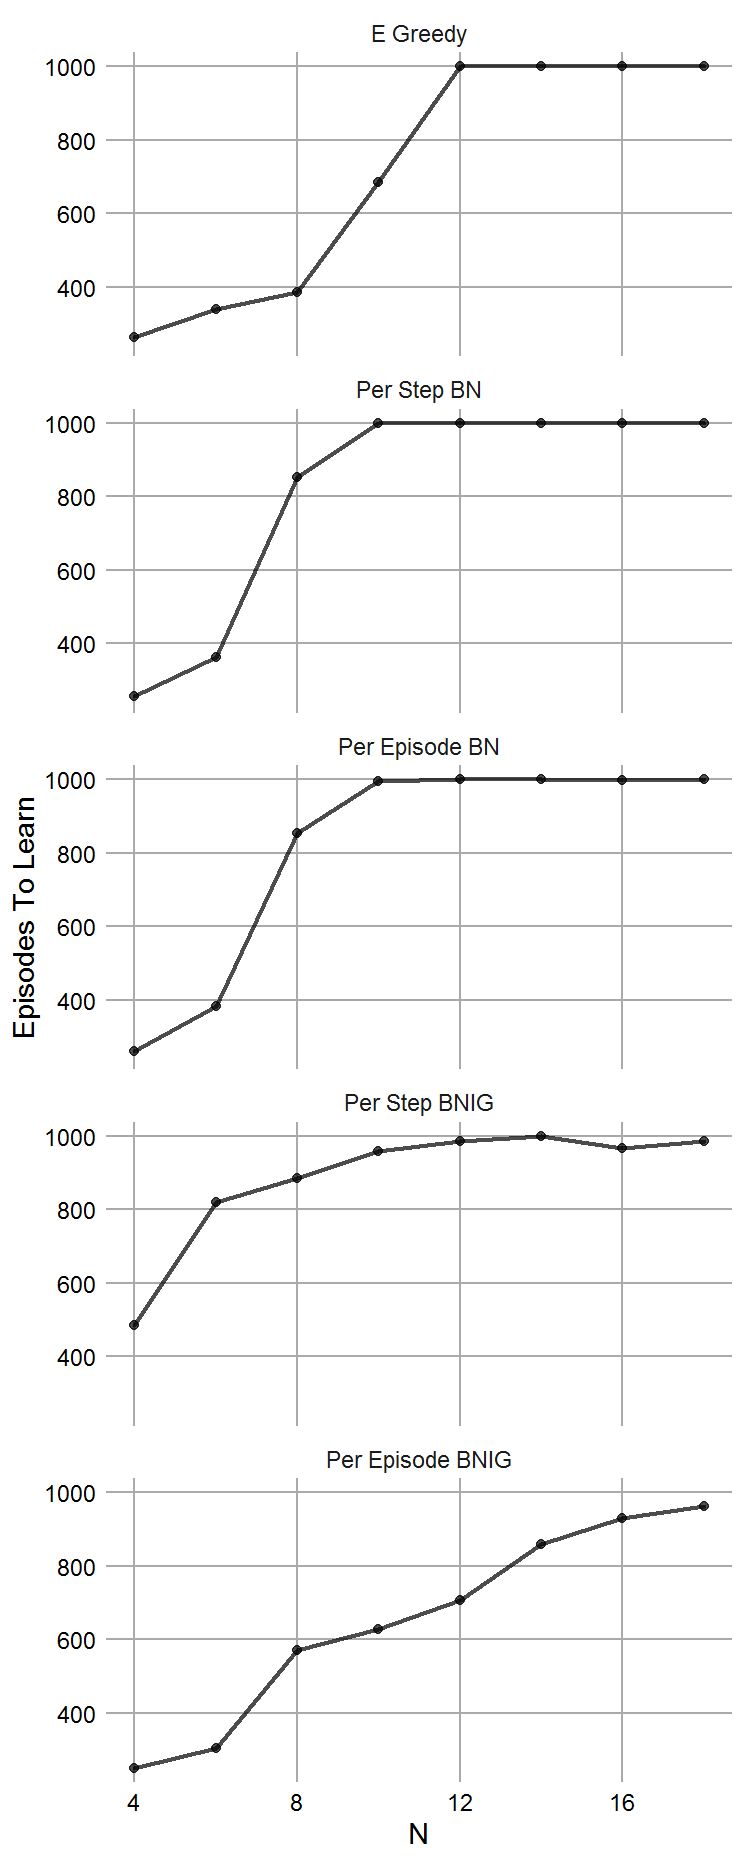
\includegraphics[scale=0.5]{Corridor1StepMethods.png}
    }
    \subfloat[3 step update]{
        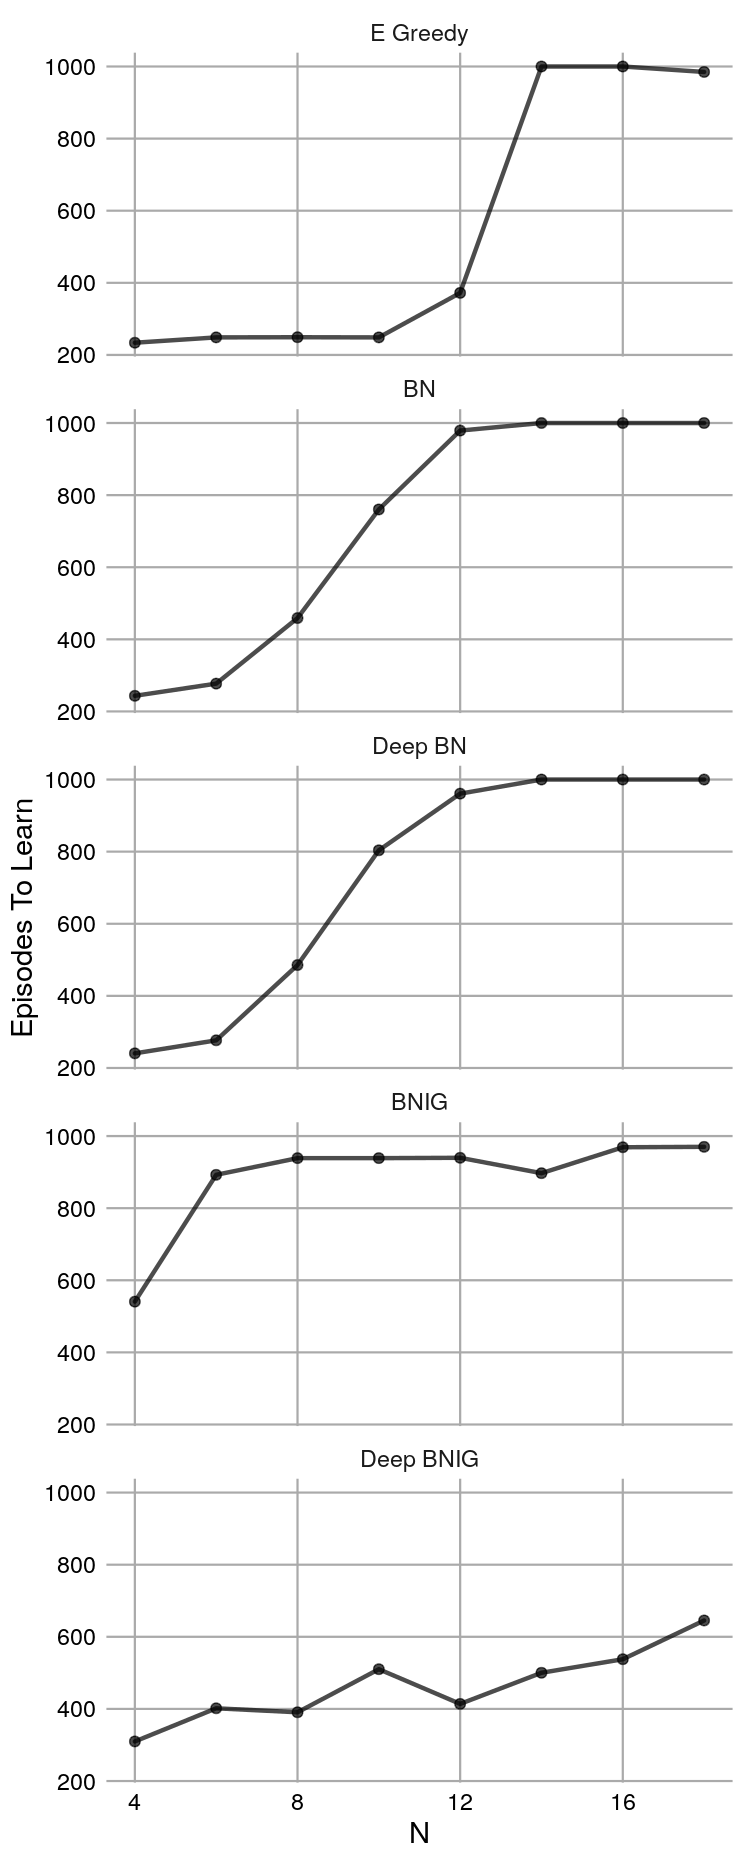
\includegraphics[scale=0.5]{Corridor3StepMethods.png}
    }
    \caption{\textbf{Linear Model Performance on Corridor Environment}: (\textbf{a}) shows that the only method to out perform is the Deep BNIG model. Increasing to a 3-step update in (\textbf{b}) improves the performance of all models but the largest increase in performance seems to be Deep BNIG.}
    \label{fig:linear_corridor}
\end{figure}

The key result from figure \ref{fig:linear_corridor} is that the $\varepsilon$-greedy method outperforms all methods apart from the BNIG model with deep exploration. However there are a few interesting differences in the results between the bayesian models and their exploration methods. 

The regular BNIG model performs worse than the regular BN model. One reason for this could be the constant noise term allowing for exploration even when the model is certain about it's current estimate. If the BNIG model quickly learns that a left moving policy gives a reward, the variance for the left action might approach zero before it gets enough data showing that a right moving policy gives a higher reward. A BN model will result in the same issue, but the small additional variance might provide enough exploration to manage a slightly longer corridor. This effect could be counteracted in the BNIG model by making the variance term $\sigma_a^2$ dependent on the state.

Adding deep exploration has seemingly no effect on the BN model but leads to far better results on the BNIG model. This could be due to the BN model not propagating variance which quickly leads to a low variance model. Once the variance is low the difference between sampled action-value functions is also small so sampling each step versus sampling each episode will lead to similar actions.

Finally, increasing from a 1-step to a 3-step update leads to better performance across all models. However for all models apart from deep BNIG the improvement is increasing the longest learnable corridor by around 2-4 states. In deep BNIG's case the improvment is an increase of atleast 8 states and possibly more. Once again this is probably due to the BNIG model being the only one actually propagating uncertainty. By increasing the step update in the BNIG model one is not only decreasing the bias of the expected value but also decreasing the bias of the variance. In other words the n-state update not only improves the value estimation but also improves the exploration, resulting in a larger improvment than in other methods.

\section{\color{red}{Temp?} \color{black} State Dependent Inverse Gamma Distribution}

\todo This might not be worth including but I'm writing it down so we can discuss if it's worth working on.

\todo I originally worked on this to stabalize beta (which no longer is a problem) but realized it could be used with a model. I've tested a bit on corridor with a linear model with OK results, but need to test more to actually conclude that this works. But I wont work more on this until we have discussed this and after I've come further on my thesis.

The variance of a state should be dependent on the state, which is not the case with in BNIG model. To fix this the inverse gamma distribution parameters should be dependent on the state. With some linear algebra it is possible to rewrite the $b$ term in terms of the next state variance and temporal difference. First recall the parameter updates

\begin{align}
    a_n &= a_0 + \frac{n}{2} \\
    b_n &= b_0 + \frac{1}{2}(Q^TQ - \mu_n^TX^TX\mu_n)
\end{align}

where some terms are removed as a prior mean of 0 is used.

Denote $y$ as the target, $\hat{Q}$ as the action-value of the next state and $Q$ the action-value of the current state. The target is then distributed by $N(r + \hat{Q}, \sigma^2_{a'})$. Using the moments of a normal distribution one finds

\begin{equation}
    \begin{split}
        \mathbb{E}[Q^TQ] &= n\sigma^2_{a'} + (r + \hat{Q})^T(r + \hat{Q})\\
        \mathbb{E}[b_n] &= b_0 + \frac{1}{2}\bigg(n\sigma^2 + (r + \hat{Q})^T(r + \hat{Q}) - Q^TQ\bigg)\\
        &= b_0 + \frac{1}{2}\bigg(n\sigma^2_{a'} + (r + \hat{Q} - Q)^T(r + \hat{Q} + Q)\bigg)\\
        &= b_0 + \frac{1}{2}\bigg(n\sigma^2_{a'} + \delta^T(r + \hat{Q} + Q)\bigg)\\
        &= b_0 + \frac{1}{2}\bigg(n\sigma^2_{a'} + 2\delta^Ty-\delta^T\delta\bigg)
    \end{split}
\end{equation}

where $\delta$ is the temporal difference and the last line reduces the number arguments required for the calculation. This leaves an equation that is dependent on the variance of the next state and the temporal difference error. With this setup $\sigma^2_a$ can be replaced by a model $\sigma^2_{a} = X\beta_{\sigma_{a}}$ that trains on targets $\sigma^2_{a'} + 2\delta^Ty-\delta^T\delta$.

\cleardoublepage